\documentclass[12pt]{article}

% Packages
\usepackage[a4paper, margin=1in]{geometry}
\usepackage{setspace}
\usepackage{graphicx}
\usepackage{amsmath}
\usepackage{booktabs}
\usepackage{array}
\usepackage{tabularx}
\usepackage[table]{xcolor}
\usepackage{hyperref}
\usepackage{float}
\usepackage[authoryear]{natbib}

\onehalfspacing

\begin{document}

\begin{titlepage}
\centering

% Logo

\includegraphics[width=0.2\textwidth]{figures/logo.png}\par\vspace{1cm}

{\Large \textbf{Beyond Employment: A Multi-Dimensional Evaluation of MGNREGA in India}}\\[0.4cm]
{\large A Panel Data Analysis of Welfare, Equity, and Efficiency Trade-offs}\\[1.2cm]

\textbf{Authors:}\\[0.3cm]
Tanishq Gupta (22322031)\\
Kavish Jain (22322017)\\
Tushar Singh (22322032)\\
Yash Kumar (22322034)\\[1cm]

\textbf{Institution Name}\\
HSS / Public Policy (optional)\\[1cm]

April 2026

\vfill
\end{titlepage}


\newpage
\begin{abstract}
This paper presents a multi-dimensional evaluation of the Mahatma Gandhi National Rural Employment Guarantee Act (MGNREGA) using a district-level panel dataset spanning 2014–2024. Unlike traditional studies that focus on a single outcome, we develop a five-pillar framework capturing shock absorption, distributional equity, income effects, labor market distortion, and structural persistence.

Using fixed-effects panel regressions and normalized index construction, we quantify the performance of MGNREGA across these dimensions and aggregate them into a composite welfare index. Our findings suggest that while MGNREGA significantly enhances income and provides resilience during economic shocks, its distributional effectiveness remains uneven and efficiency trade-offs emerge in certain regions.

The analysis further highlights substantial regional heterogeneity and a shift in program dynamics during the COVID-19 period, where MGNREGA functioned primarily as a stabilization mechanism rather than a development tool. Overall, the results indicate that MGNREGA functions primarily as a counter-cyclical income stabilization mechanism, with heterogeneous effects across regions and measurable trade-offs between welfare gains and productive efficiency.
\end{abstract}

\newpage
\newpage

\tableofcontents
\newpage

\section{Introduction}

The Mahatma Gandhi National Rural Employment Guarantee Act (MGNREGA) is one of the largest public employment programs in the world, designed to provide livelihood security through guaranteed wage employment in rural India. Since its implementation in 2005, the program has been widely studied for its impact on rural wages, consumption, poverty alleviation, and labor markets. Early empirical work suggests that MGNREGA has contributed to increasing rural wages and reducing distress migration, particularly among vulnerable households \cite{ImbertPapp2015, Berg2012}. At the same time, concerns have been raised regarding potential labor market distortions and inefficiencies arising from public employment schemes \cite{Muralidharan2017}.

Despite a large body of empirical work, most studies on MGNREGA examine isolated outcomes—such as wages, consumption, or migration—without integrating these effects into a unified evaluative framework. This fragmented approach limits our understanding of the overall welfare implications of the program, particularly in the presence of trade-offs between equity, efficiency, and resilience.

A parallel strand of literature in development economics emphasizes the importance of evaluating policies through multiple channels, including resilience, equity, and efficiency \cite{BanerjeeDuflo2011}. In particular, public employment programs are often conceptualized not only as income-support mechanisms but also as tools for insurance against income shocks and as instruments for structural transformation in rural economies. However, empirical frameworks that jointly capture these dimensions remain limited.

This paper seeks to address this gap by developing a comprehensive, multi-dimensional evaluation framework for MGNREGA. Using a district-level panel dataset spanning 2014–2024, we construct five key pillars of policy impact: (1) shock absorption, capturing the program’s ability to stabilize income during adverse rainfall shocks; (2) distributional equity, measuring differential benefits across marginalized groups; (3) income effects, reflecting overall welfare gains; (4) labor market distortion, capturing trade-offs between income gains and productive efficiency; and (5) structural persistence, assessing the extent to which MGNREGA generates lasting economic effects.

Methodologically, the analysis employs fixed-effects panel regressions to estimate the contribution of MGNREGA across each pillar, followed by normalization and aggregation into a composite index. This approach allows for a unified comparison of policy performance across regions and over time, as well as an examination of trade-offs between welfare, equity, and efficiency.

Our findings reveal that MGNREGA functions primarily as an income-support and stabilization mechanism, with significant variation across regions and economic conditions. In particular, the program exhibits stronger performance during periods of economic stress, such as the COVID-19 pandemic, where its role shifts toward short-term relief rather than long-term structural transformation. At the same time, distributional gains remain uneven, and evidence of efficiency trade-offs emerges in certain contexts.

This paper contributes to the literature in three ways. First, it proposes a unified multi-dimensional evaluation framework that jointly captures welfare, equity, efficiency, and dynamic persistence. Second, it provides district-level panel evidence on the heterogeneous and time-varying effects of MGNREGA. Third, it explicitly quantifies trade-offs between income support and productive efficiency, which are often overlooked in single-outcome analyses.

The remainder of the paper is structured as follows. Section 2 presents the conceptual framework underlying the five pillars of analysis. Section 3 describes the data and variable construction. Section 4 outlines the empirical methodology. Section 5 presents the results, followed by economic interpretation and policy implications in Section 6. Section 7 concludes.

\section{Conceptual Framework}

Evaluating a large public policy like MGNREGA using a single outcome can often give an incomplete picture. For example, a program may increase income but at the same time create inefficiencies in labor markets or fail to benefit all social groups equally. Because of this, recent work in development economics has increasingly emphasized the need to look at policies from multiple dimensions rather than focusing on just one metric \citep{BanerjeeDuflo2011}.

In this paper, we propose a five-pillar framework to evaluate the impact of MGNREGA in a more holistic way. Each pillar captures a different economic channel through which the policy operates. Together, they provide a more balanced understanding of the program’s overall impact.

\subsection{Shock Absorption (Resilience)}

One of the key roles of employment guarantee programs is to act as a safety net during times of economic distress. In rural India, rainfall shocks can have a direct impact on agricultural income and household consumption. MGNREGA is expected to provide an alternative source of income during such periods, helping households smooth their consumption.

This idea is closely related to the broader concept of informal insurance in developing economies, where public programs substitute for missing credit and insurance markets \citep{Townsend1994}. In this context, a strong shock absorption effect would mean that MGNREGA helps reduce the negative impact of adverse shocks on income.

\subsection{Distributional Equity}

Another important objective of MGNREGA is to improve equity by targeting marginalized groups, including Scheduled Castes (SC), Scheduled Tribes (ST), and women. Several studies have shown that access to public employment can improve bargaining power and participation for disadvantaged groups \citep{Duflo2012}.

In our framework, the distributional pillar captures whether the benefits of MGNREGA are shared equally across different social groups or whether they are concentrated among specific segments of the population. A stronger distributional effect would indicate that the program is inclusive and equitable.

\subsection{Income Effect (Welfare)}

At its core, MGNREGA is designed to increase rural income by providing wage employment. A large part of the existing literature focuses on this channel, examining whether the program leads to higher household income and consumption \citep{ImbertPapp2015}.

In this study, the income pillar captures the overall welfare impact of MGNREGA. A positive income effect would suggest that the program is successful in raising living standards, while a weaker effect may indicate limited economic benefits.

\subsection{Labor Market Distortion (Efficiency)}

While MGNREGA can increase income, it may also affect labor markets in unintended ways. For example, by setting a wage floor, the program may reduce the supply of labor available for agricultural work or increase wages in the private sector. This can create efficiency losses if it leads to a decline in agricultural productivity.

This concern has been highlighted in earlier work on public employment programs, which points to potential trade-offs between welfare gains and market efficiency \citep{Muralidharan2017}. In our framework, the distortion pillar captures this trade-off by comparing income gains with changes in productive outcomes.

\subsection{Structural Persistence (Dynamic Effects)}

Finally, an important question is whether the effects of MGNREGA last beyond the immediate period. Does the program lead to sustained improvements in income, or are the benefits short-lived?

We capture this idea through what we call structural persistence. Rather than focusing only on immediate effects, this pillar looks at whether MGNREGA has lagged impacts on income and economic activity. A strong persistence effect would suggest that the program contributes to longer-term stability, even if it does not directly transform productivity.

\subsection{Bringing the Five Pillars Together}

These five pillars—shock absorption, distribution, income, distortion, and structural persistence—are not independent of each other. In many cases, they interact and create trade-offs. For instance, a policy that strongly increases income may also generate higher distortion, while a program that improves equity may not always maximize efficiency.

By combining all five dimensions into a unified framework, this paper aims to provide a more complete evaluation of MGNREGA. Instead of asking whether the program “works” in a single sense, we ask how it performs across multiple dimensions and how these dimensions evolve over time and across regions.


\section{Data and Variable Construction}

This study is based on a district-level panel dataset constructed by combining multiple sources of data related to income, consumption, agriculture, demographics, rainfall, and MGNREGA program outcomes. The final dataset covers 293 districts over the period 2014 to 2024, resulting in a balanced panel with 3,223 observations.\footnote{The final panel is constructed as a strict intersection of all data sources to ensure consistency across variables.}

\subsection{Data Sources and Coverage}

The dataset brings together information from several sources. Household-level income and consumption data are obtained from CMIE Consumer Pyramids, while agricultural data is taken from the Directorate of Economics and Statistics. Rainfall data is sourced from the Indian Meteorological Department (IMD), and poverty indicators are obtained from NITI Aayog’s district-level MPI estimates. MGNREGA-related variables are collected through web scraping of official government portals.

Since these datasets differ in coverage and structure, the final panel is constructed by taking the common intersection across all sources. As a result, the number of districts in the final dataset is lower than the original coverage of individual sources, but ensures that all variables are consistently available for each district-year observation.

The panel structure enables exploitation of within-district variation over time, which is central to the identification strategy employed in this study.

\subsection{Income and Consumption Variables}

Income data is constructed using household-level CMIE records. Monthly observations are first converted into annual values, and a weighted average is computed at the district-year level using household weights. The final variable used in the analysis is total district-level income.

Similarly, consumption is measured using household expenditure data, with a focus on adjusted total expenditure. These values are aggregated to the district-year level to capture overall consumption patterns.

\subsection{Agricultural Outcomes}

Agricultural data is compiled from crop-level district datasets covering major crops such as rice, cotton, pulses, and sugarcane. After cleaning and standardizing the data, total production and total cultivated area are calculated for each district-year. These are then used to construct an agricultural yield index, defined as total production divided by total area.

This index provides a simple but useful measure of agricultural productivity across districts and over time.

\subsection{Rainfall Data}

Rainfall plays a key role in this study as a source of exogenous variation. Annual rainfall data is constructed using gridded IMD datasets. Daily rainfall values are aggregated to annual totals and then mapped to districts using spatial boundaries.

The resulting variable captures total annual rainfall (in millimeters) for each district and year.

\subsection{MGNREGA Variables}

MGNREGA data is collected through a custom web scraping pipeline that extracts district-level information from official government reports. The data includes employment indicators, wage payments, participation of SC/ST workers, and female participation rates.

Several cleaning steps are applied to handle missing values, inconsistent district naming, and reporting gaps. In cases of limited missingness, interpolation is used cautiously to preserve panel continuity. Robustness checks excluding interpolated observations yield qualitatively similar results (Appendix D).

\subsection{Demographics and Poverty Indicators}

District-level demographic variables, including rural population and area, are obtained from Census 2011 data. Poverty indicators are sourced from NITI Aayog’s Multidimensional Poverty Index (MPI).

These variables are treated as time-invariant and merged with the panel dataset after construction.

\subsection{Panel Construction}

The final panel dataset is built through a series of careful merging and cleaning steps. District names are standardized across datasets, and alias mappings are used to resolve inconsistencies. Only districts with complete data across all years are retained to ensure a balanced panel.

The merging process follows a sequential approach, combining MGNREGA data with agriculture, asset ownership, rainfall, income, and consumption variables. Static variables such as population and MPI are then added.

Several quality checks are performed during this process, including duplicate checks, missing value diagnostics, and consistency checks across years. The final dataset contains all variables required for the multi-dimensional analysis carried out in this paper.

\subsection{Final Dataset Overview}

The final dataset is an annual district-level panel covering 293 districts across 11 years (2014–2024). It includes variables related to:

\begin{itemize}
\item MGNREGA employment, wages, and participation
\item Income and consumption
\item Agricultural production and yield
\item Rainfall
\item Asset ownership
\item Demographics and poverty indicators
\end{itemize}

This integrated dataset forms the basis for the empirical analysis presented in the following sections.

\section{Exploratory Data Analysis}

Before moving to the empirical analysis, it is useful to examine the basic patterns in the data. This section presents key descriptive trends related to employment, wages, expenditure, and socio-economic outcomes under MGNREGA. The goal is to build intuition and highlight broad patterns that later help interpret the regression results.

\subsection{Trends in Employment and Participation}

\begin{figure}[H]
\centering
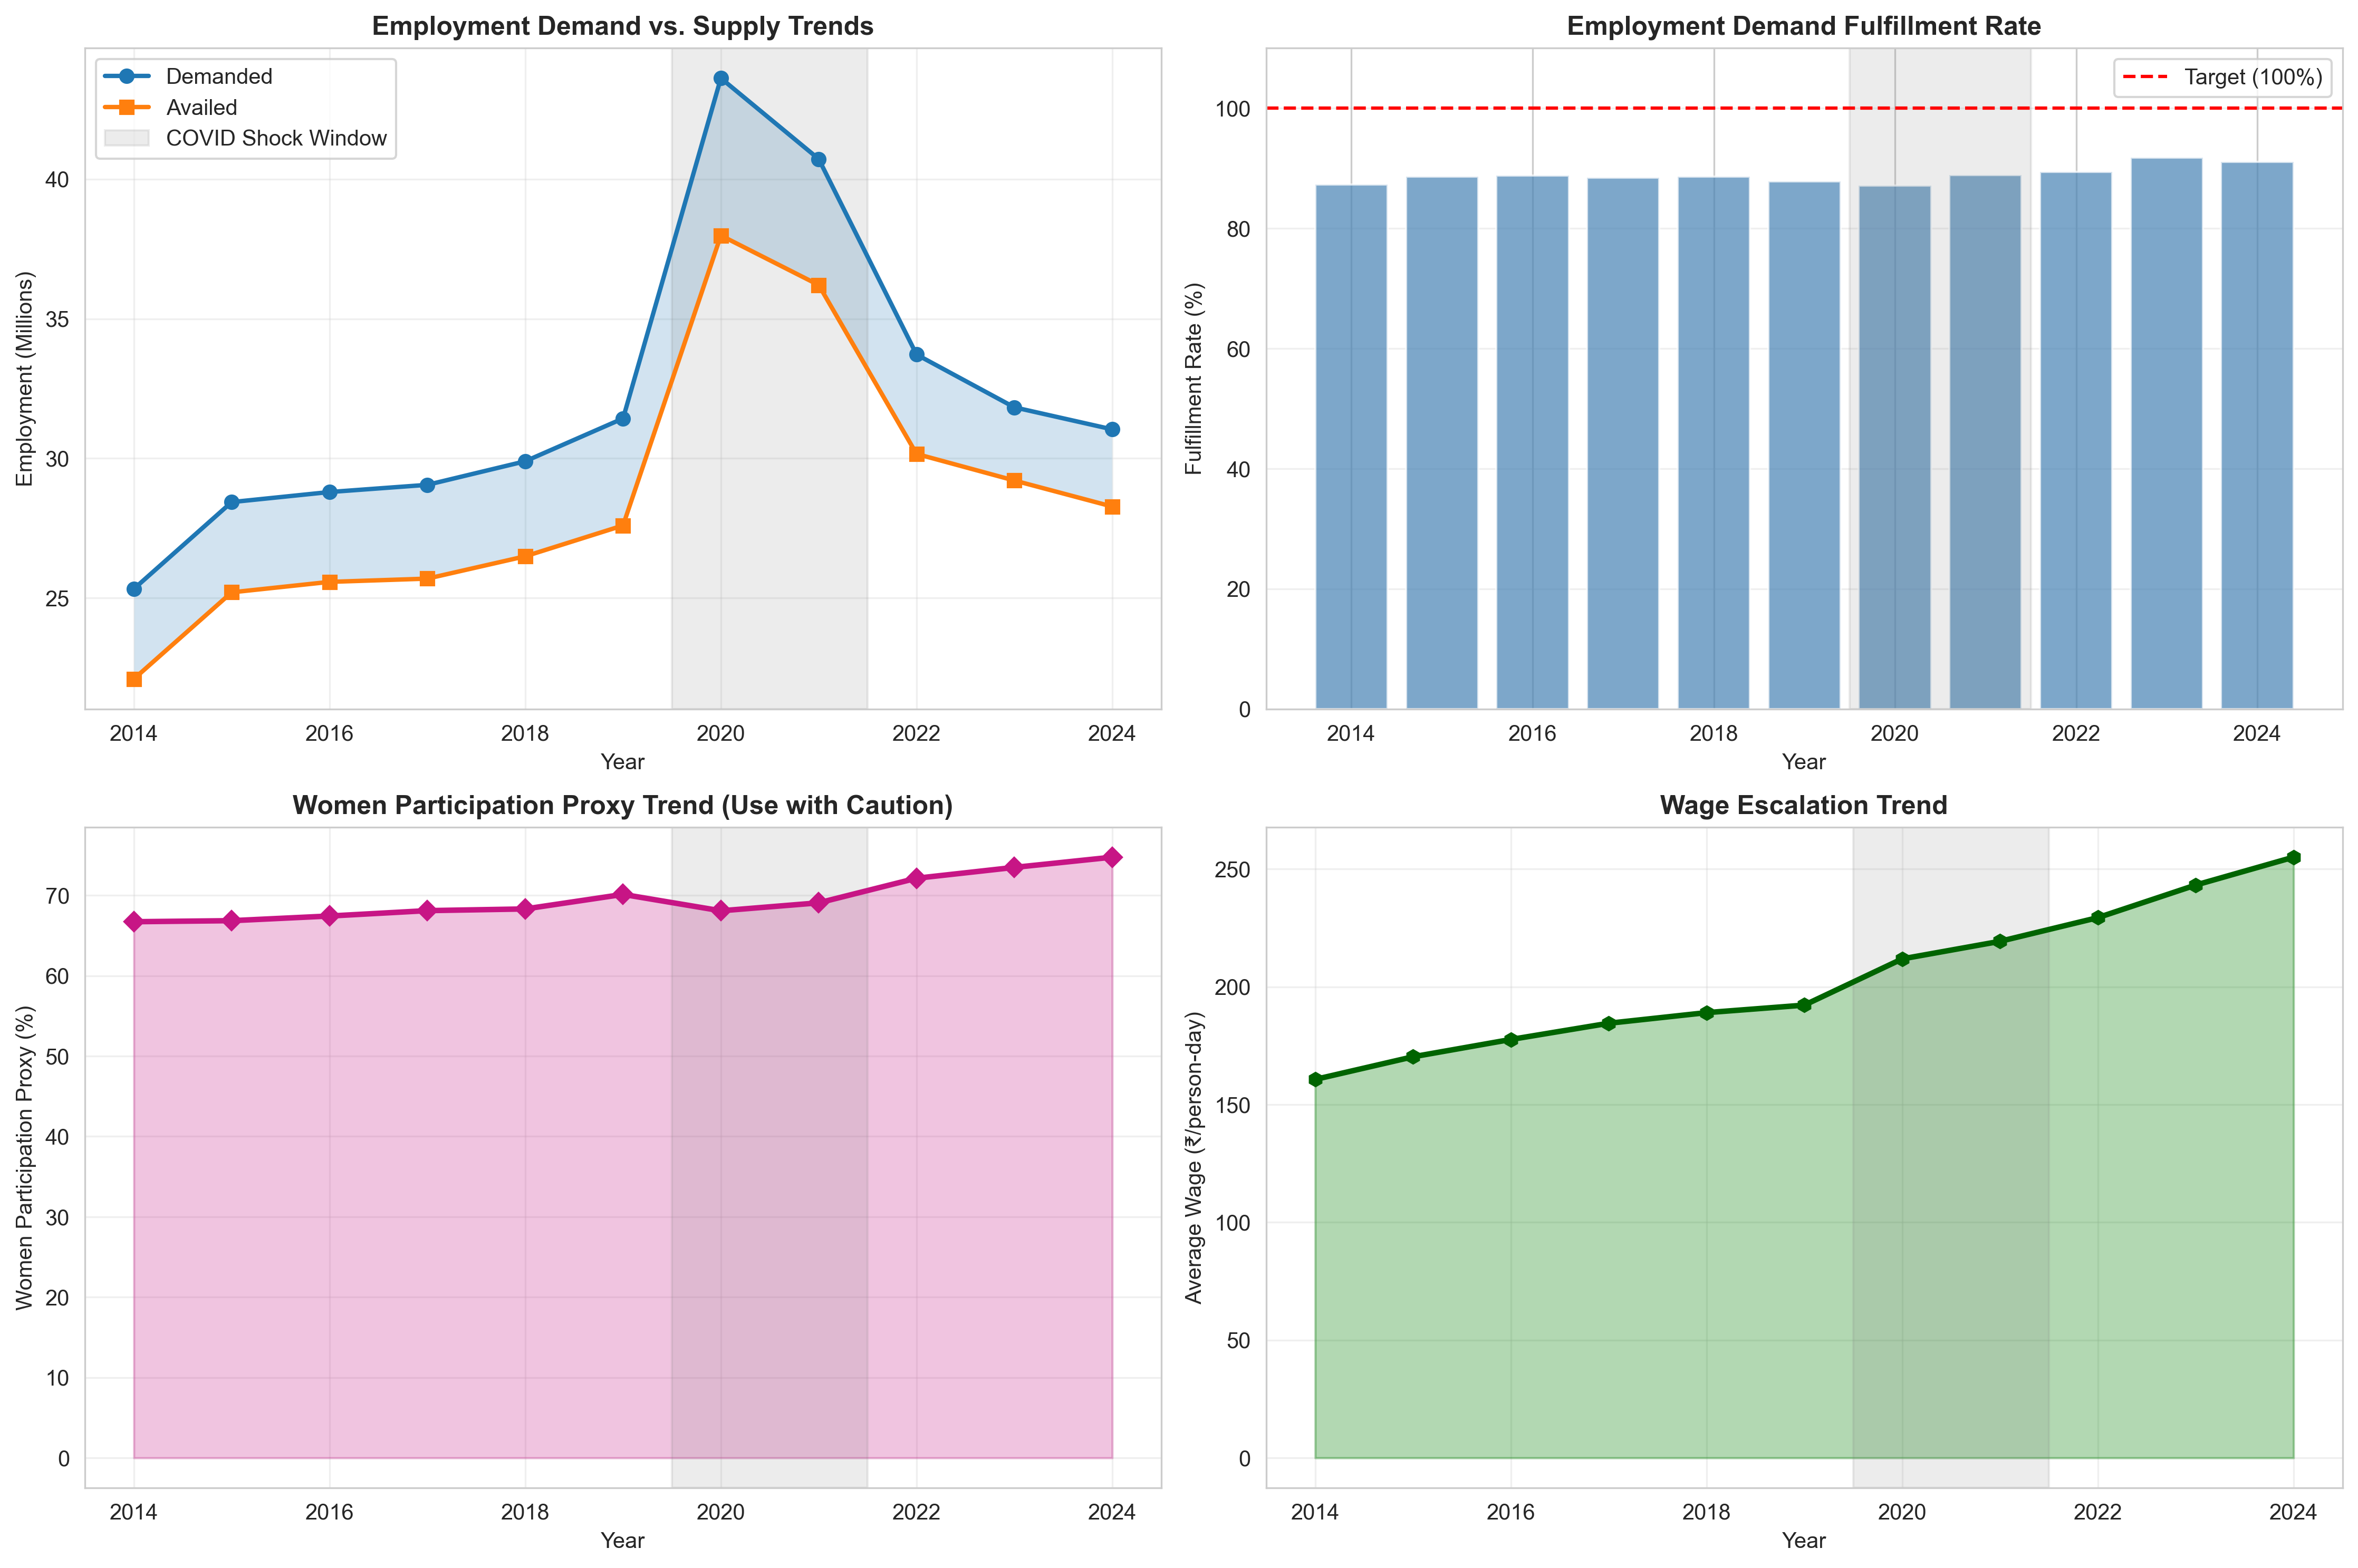
\includegraphics[width=0.9\textwidth]{figures/figure11.png}
\caption{Temporal trends in employment demand, availed employment, fulfilment rates, women participation, and wages.}
\label{fig:trends}
\end{figure}

Figure \ref{fig:trends} shows the evolution of employment demand and availed employment over time. A clear increase is visible during the COVID-19 period, where both demand and actual employment rise sharply. This suggests that MGNREGA acted as an important fallback option during economic stress.

At the same time, the gap between demand and availed employment remains present throughout the period, indicating that full demand is not always met. The fulfilment rate remains high but below the ideal 100 percent benchmark, pointing to capacity constraints in implementation.

The figure also shows a steady rise in wages over time. Women’s participation, measured through a proxy variable, shows an upward trend as well, although it should be interpreted with caution given data limitations.

\subsection{Fiscal Expansion and Wage Dynamics}

\begin{figure}[H]
\centering
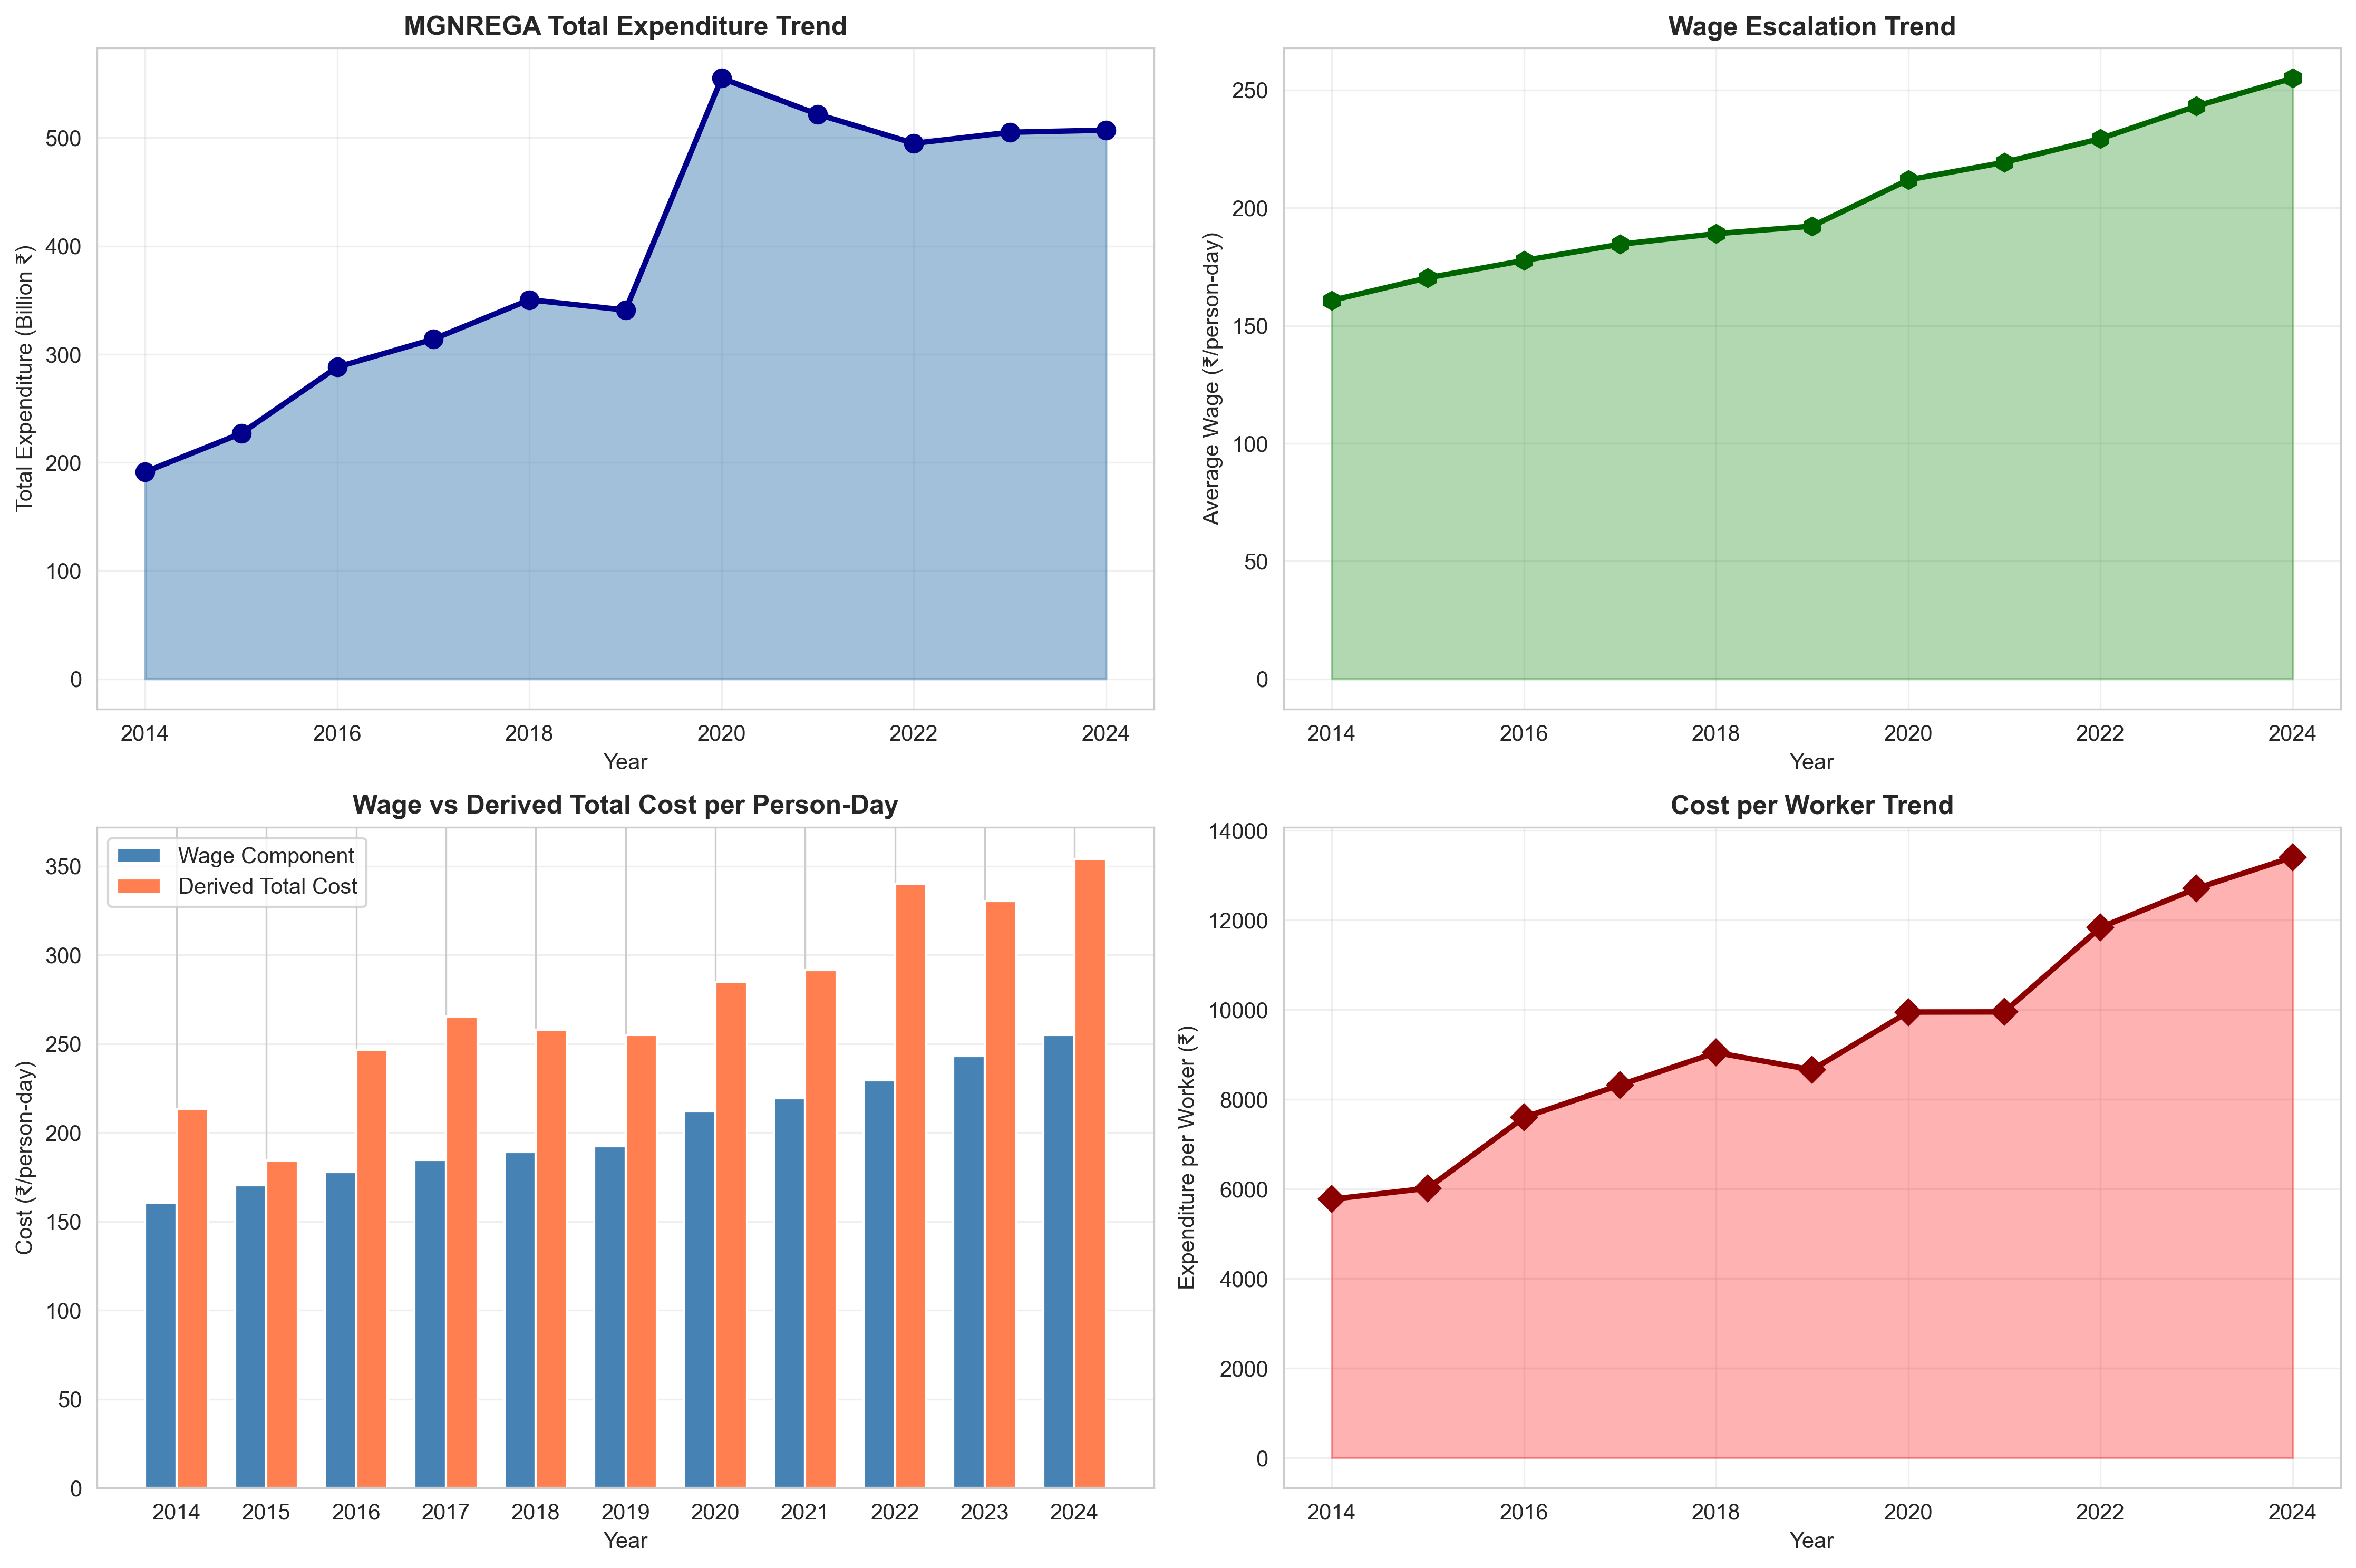
\includegraphics[width=0.9\textwidth]{figures/figure4.png}
\caption{Expenditure trajectory, wage growth, and cost per worker under MGNREGA.}
\label{fig:fiscal}
\end{figure}

Figure \ref{fig:fiscal} highlights the financial side of the program. Total expenditure increases significantly over time, with a sharp jump during the COVID period. This is consistent with the increase in employment demand observed earlier.

Wages also show a consistent upward trend, suggesting that MGNREGA may be contributing to a rising wage floor in rural labor markets. However, the cost per worker also increases, which raises questions about efficiency and fiscal sustainability.

These patterns are important for understanding the income and distortion effects of the program, which are explored in later sections.

\subsection{Income, Productivity, and Asset Trends}

\begin{figure}[H]
\centering
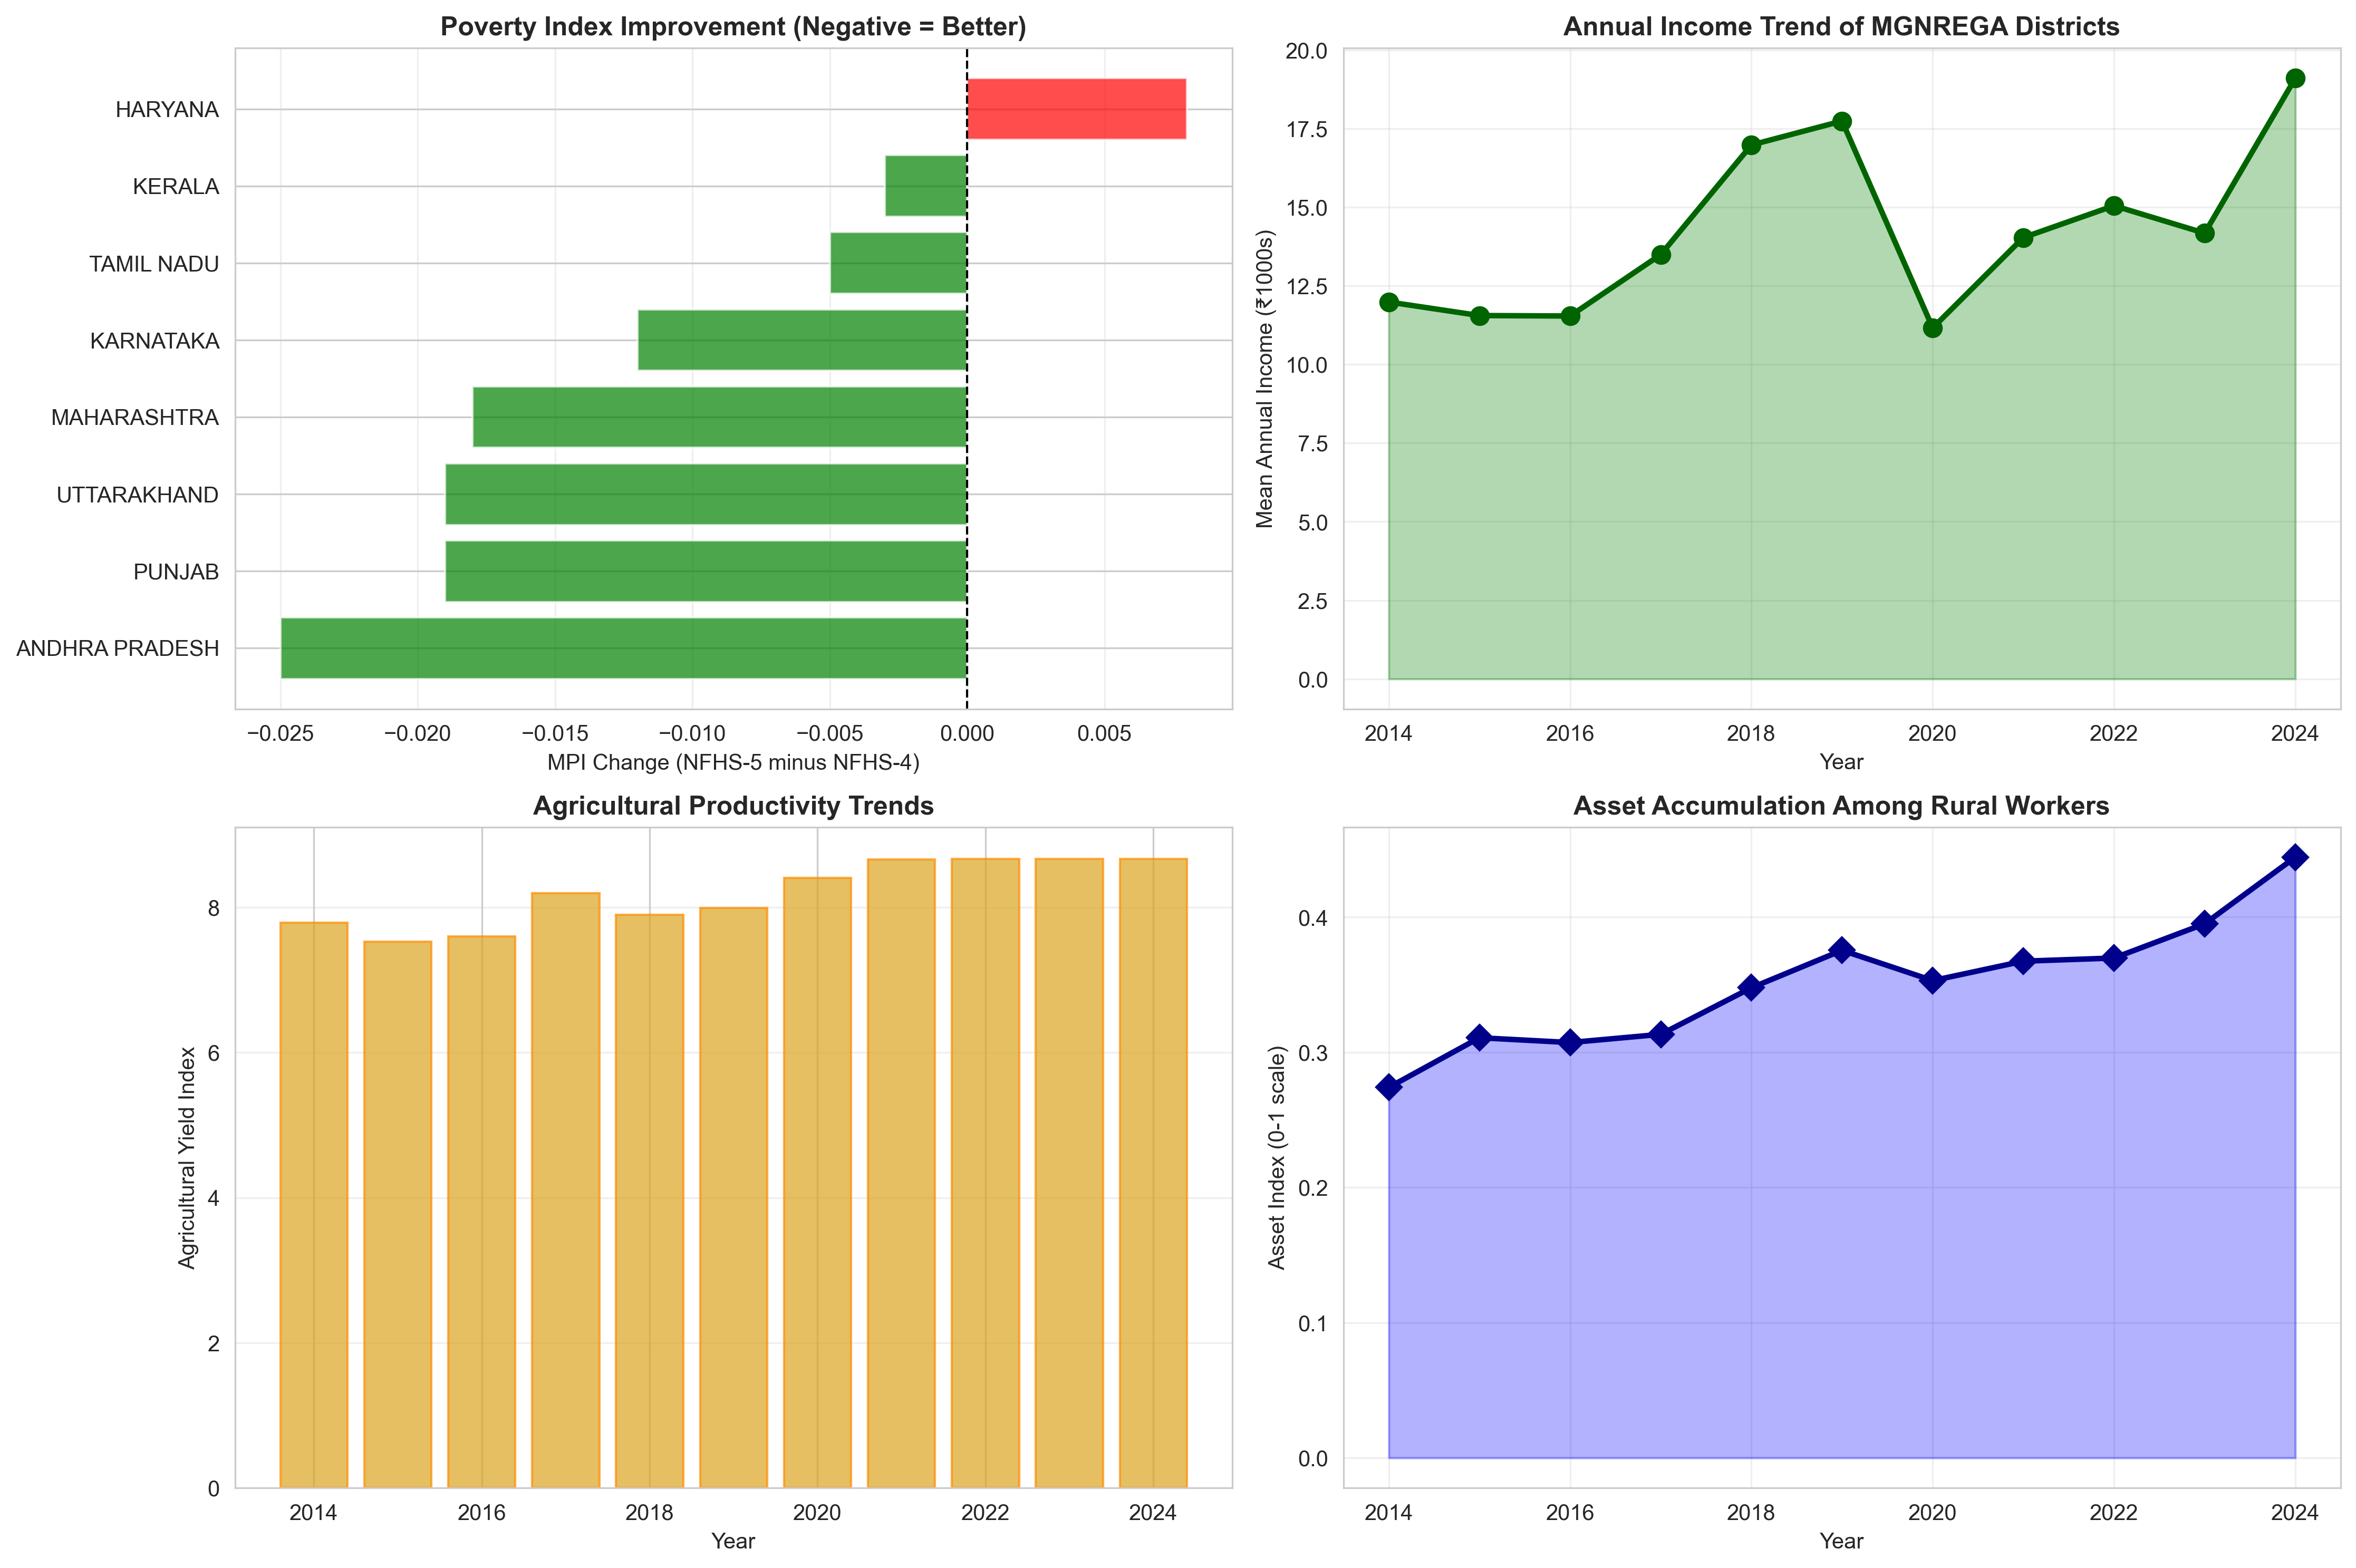
\includegraphics[width=0.9\textwidth]{figures/figure5.png}
\caption{Income trends, agricultural productivity, poverty transitions, and asset accumulation.}
\label{fig:income}
\end{figure}

Figure \ref{fig:income} brings together key indicators related to income, agriculture, and long-term outcomes. Average income shows an overall increasing trend, although there is a noticeable dip during the COVID period followed by recovery.

Agricultural productivity, measured through the yield index, shows relatively stable growth over time. This suggests that while MGNREGA increases income, its direct impact on agricultural productivity may be limited.

The asset index shows gradual improvement, indicating some degree of accumulation over time. At the same time, changes in the poverty index suggest modest improvements in welfare, though the magnitude varies across regions.

Together, these patterns point toward income gains and some persistence effects, but not necessarily strong structural transformation.

\subsection{Correlation Patterns and Distribution Across Districts}

\begin{figure}[H]
\centering
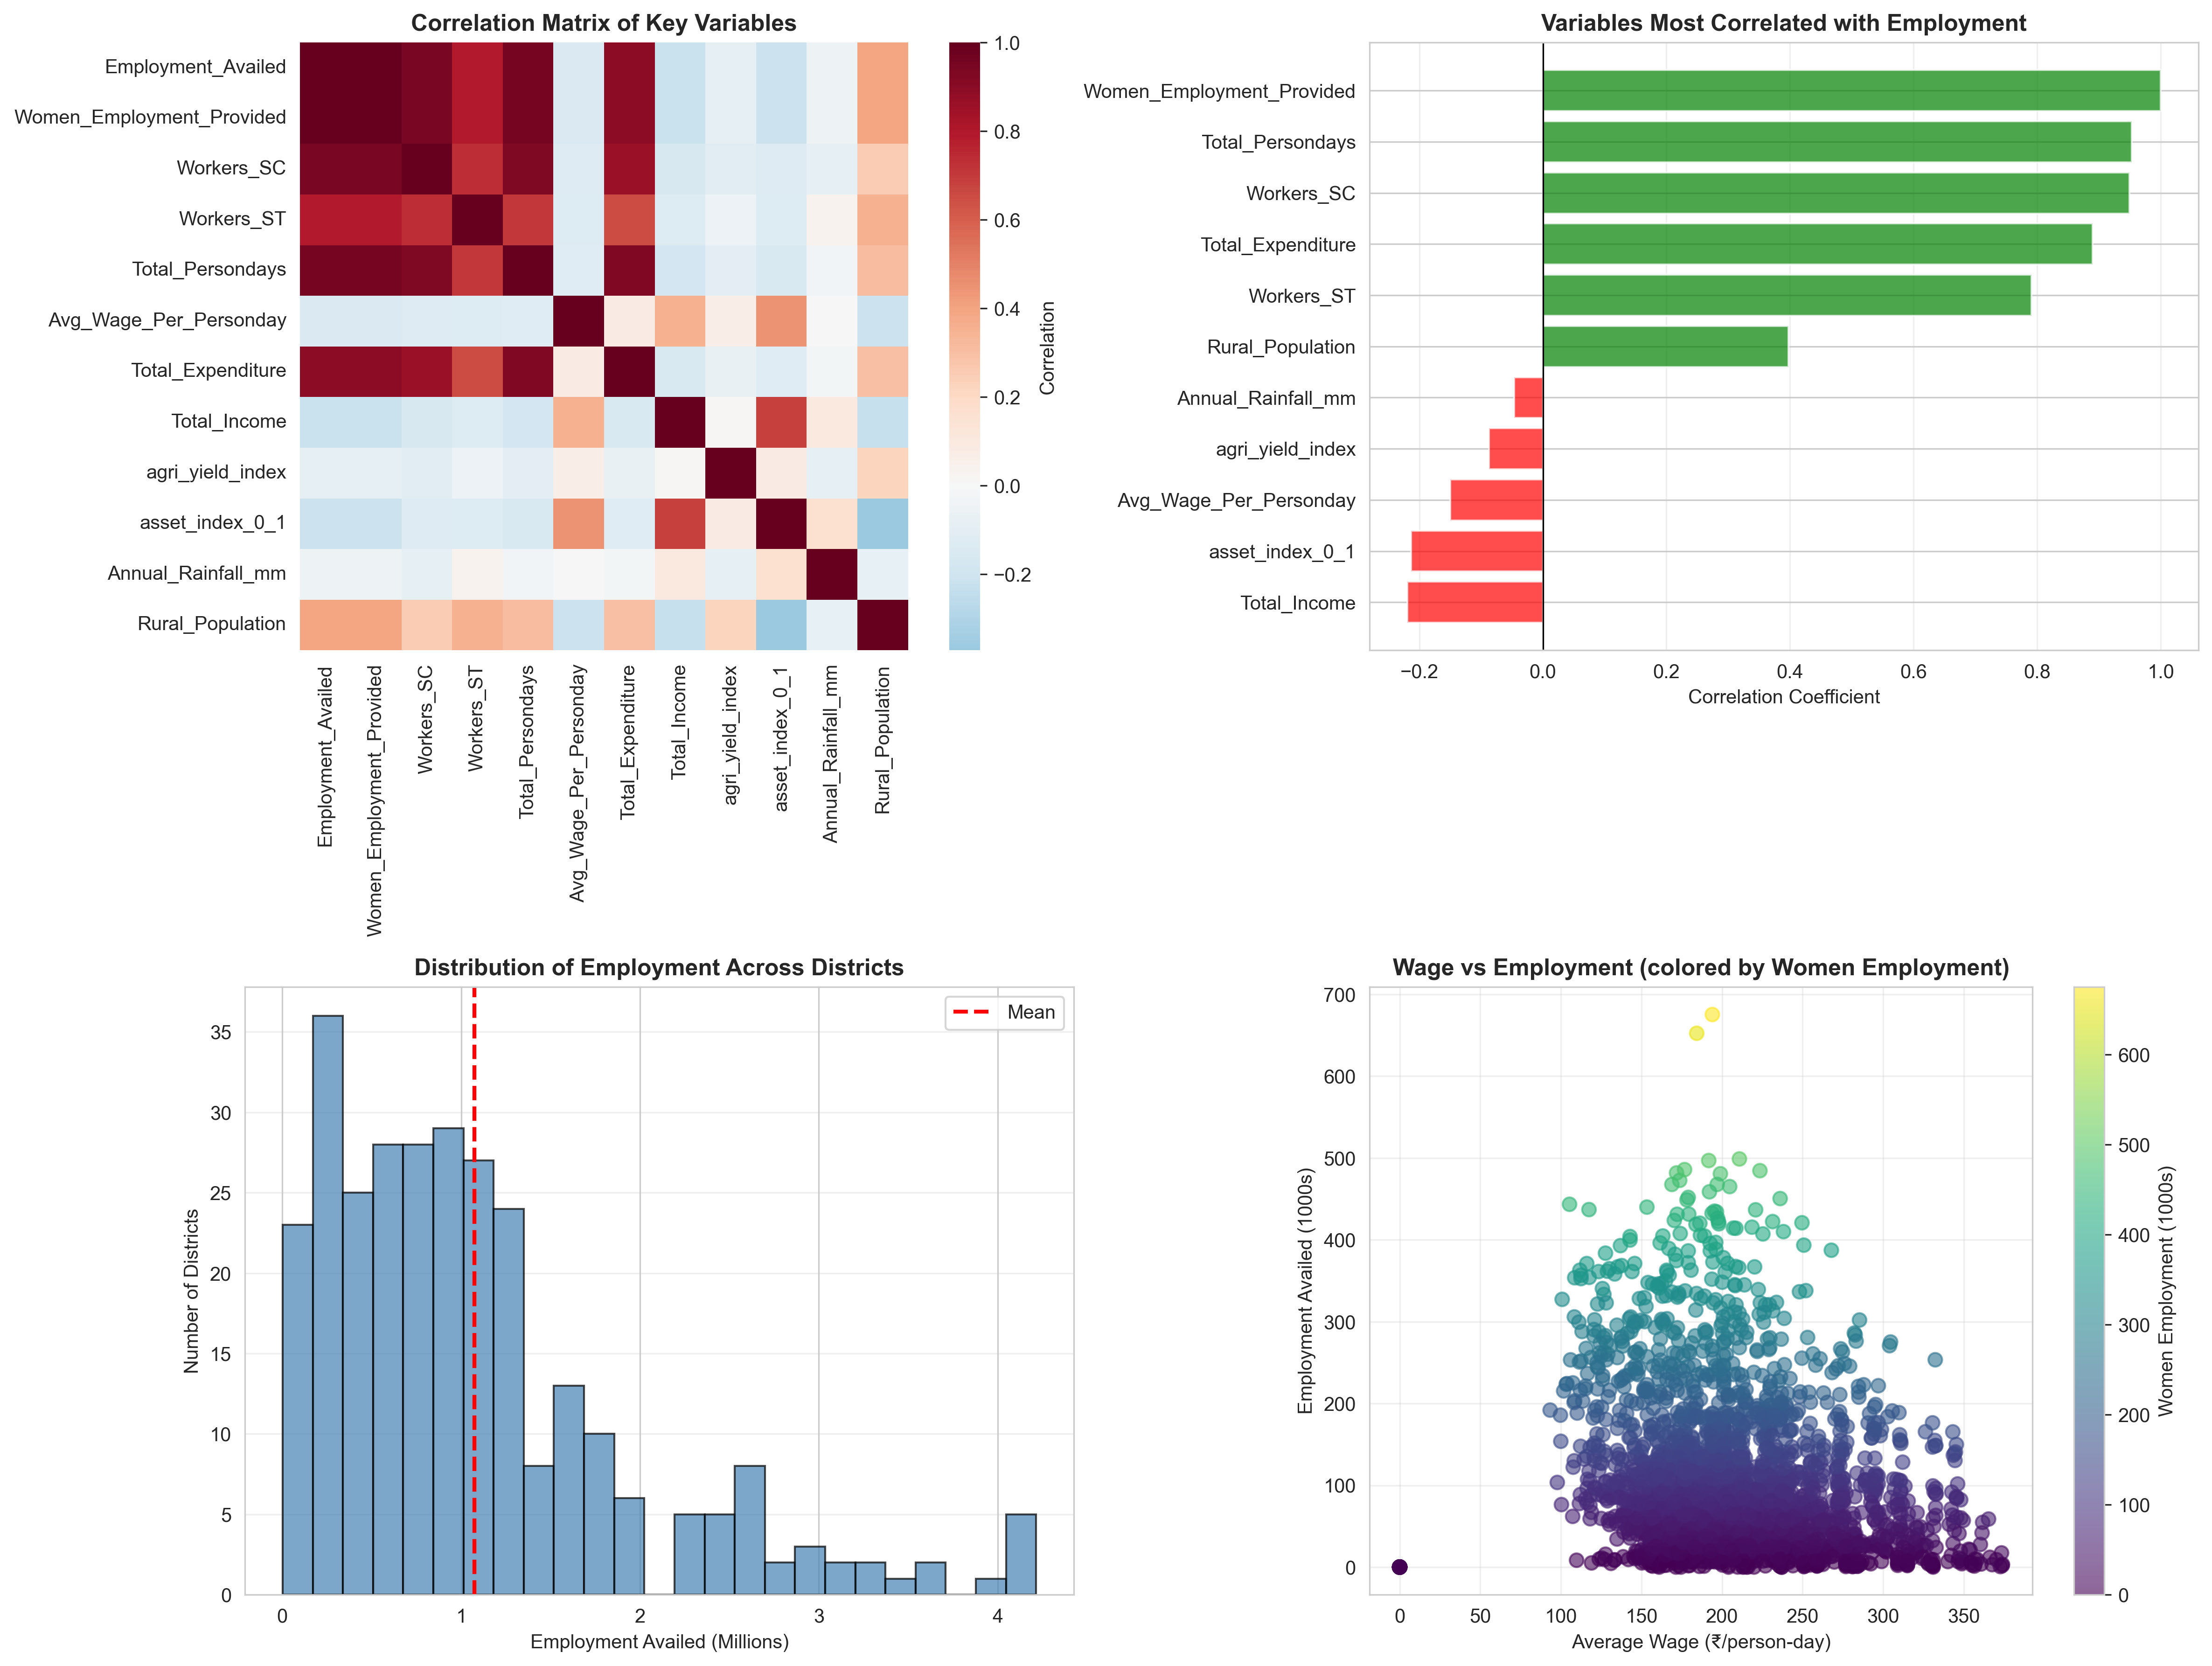
\includegraphics[width=0.9\textwidth]{figures/figure6.png}
\caption{Correlation structure and distribution of employment across districts.}
\label{fig:correlation}
\end{figure}

Figure \ref{fig:correlation} provides additional insight into how key variables are related. Employment is strongly correlated with variables such as total expenditure and person-days, which is expected given the design of the program.


At the same time, the distribution of employment across districts shows considerable variation. While some districts consistently generate high levels of employment, others remain below the average. This highlights the importance of regional heterogeneity in understanding program outcomes.

The scatter plot also suggests a relationship between wages and employment, although the pattern is not perfectly linear. This indicates that wage increases do not uniformly translate into higher employment across all districts.

\subsection{Summary of Key Patterns}

The exploratory analysis highlights several important patterns. First, MGNREGA plays a clear counter-cyclical role, with employment and expenditure rising during periods of economic stress. Second, wages and income show consistent upward trends, suggesting positive welfare effects. Third, improvements in productivity and long-term outcomes are more gradual and less pronounced. Finally, there is significant variation across districts, indicating that the impact of the program is not uniform.

These observations provide useful context for the empirical analysis that follows, where these patterns are formally tested using panel regression models.

These descriptive patterns are consistent with the hypothesis that MGNREGA operates as a counter-cyclical employment mechanism, motivating the formal econometric analysis that follows.


\section{Empirical Methodology}

This section outlines the empirical approach used to evaluate the impact of MGNREGA across multiple dimensions. Rather than focusing on a single outcome, we adopt a multi-pillar framework that captures different channels through which the policy operates. Each pillar is estimated separately using panel regression models, and the results are later combined into a composite index.

\subsection{Panel Framework}

The analysis is based on a district-level panel dataset covering the period 2014–2024. To account for unobserved heterogeneity across districts and common shocks over time, we use a fixed-effects specification of the following form:

\begin{equation}
Y_{it} = \beta \cdot MGNREGA_{it} + \gamma X_{it} + \mu_i + \lambda_t + \epsilon_{it}
\end{equation}

where $i$ indexes districts and $t$ indexes years. $Y_{it}$ represents the outcome variable of interest, $MGNREGA_{it}$ captures program intensity, and $X_{it}$ includes control variables such as rainfall and population. $\mu_i$ and $\lambda_t$ represent district and year fixed effects, respectively.

This approach helps isolate the within-district variation over time, which is commonly used in policy evaluation studies \citep{ImbertPapp2015, Muralidharan2017}.

\subsection{Pillar 1: Shock Absorption}

To examine whether MGNREGA helps households cope with adverse shocks, we focus on rainfall as an exogenous source of variation. We construct a shock variable based on deviations from district-level average rainfall.

The estimation is based on the following specification:

\begin{equation}
Income_{it} = \beta_1 MGNREGA_{it} + \beta_2 Shock_{it} + \beta_3 (MGNREGA_{it} \times Shock_{it}) + \mu_i + \lambda_t + \epsilon_{it}
\end{equation}

The interaction term $\beta_3$ captures whether the effect of MGNREGA is stronger during periods of adverse shocks. A positive and significant coefficient would indicate that the program provides insurance against income fluctuations, consistent with the idea of public works acting as a safety net \citep{Townsend1994}.


\subsection{Pillar 2: Distributional Effects}

To assess whether MGNREGA benefits are evenly distributed across social groups, we construct subgroup-specific outcome variables using the share of SC/ST workers and women participation.

We estimate separate regressions for these groups:

\begin{equation}
Y^{group}*{it} = \beta \cdot MGNREGA*{it} + \mu_i + \lambda_t + \epsilon_{it}
\end{equation}

where $Y^{group}_{it}$ represents income or employment outcomes for specific groups. This approach allows us to directly measure whether program benefits are inclusive, rather than relying only on aggregate effects.

This dimension is motivated by literature emphasizing the role of public programs in improving access and participation for disadvantaged groups \citep{Duflo2012}.

\subsection{Pillar 3: Income Effects}

The income pillar captures the overall welfare impact of MGNREGA. We estimate the following model:

\begin{equation}
Income_{it} = \beta \cdot MGNREGA_{it} + \gamma X_{it} + \mu_i + \lambda_t + \epsilon_{it}
\end{equation}

A positive coefficient on $MGNREGA_{it}$ indicates that the program increases district-level income. This is the most direct measure of welfare improvement and is widely studied in the literature \citep{ImbertPapp2015}.



\subsection{Pillar 4: Labor Market Distortion}

While MGNREGA may increase income, it can also affect labor market efficiency. To capture this trade-off, we estimate the effect of MGNREGA on both income and agricultural productivity.

We use a log-linear specification:

\begin{equation}
\log(Income_{it}) = \beta_1 MGNREGA_{it} + \mu_i + \lambda_t + \epsilon_{it}
\end{equation}

\begin{equation}
\log(Yield_{it}) = \beta_2 MGNREGA_{it} + \mu_i + \lambda_t + \epsilon_{it}
\end{equation}

We then construct a distortion measure based on the relative magnitude of $\beta_1$ and $\beta_2$. If income increases without a corresponding increase in productivity, it may indicate inefficiencies in labor allocation.

This approach reflects the broader debate on trade-offs between welfare gains and efficiency in public employment programs \citep{Muralidharan2017}.


\subsection{Pillar 5: Structural Persistence}

To examine whether the effects of MGNREGA persist over time, we estimate a model with lagged program intensity:

\begin{equation}
Income_{it} = \beta \cdot MGNREGA_{i,t-1} + \mu_i + \lambda_t + \epsilon_{it}
\end{equation}

A significant coefficient on the lagged variable suggests that the effects of MGNREGA extend beyond the current period. Rather than interpreting this as structural transformation, we view it as evidence of income persistence and dynamic effects.

\subsection{Index Construction}

After estimating each pillar, we convert the estimated effects into normalized scores. For each pillar, the estimated coefficients are scaled to lie between 0 and 1 using a min-max normalization:

\begin{equation}
Score = \frac{X - X_{min}}{X_{max} - X_{min}}
\end{equation}

These normalized scores are then combined to construct a composite index:

\begin{equation}
Index_{it} = \frac{1}{5} \sum_{k=1}^{5} Score_{k,it}
\end{equation}

We also consider a weighted version of the index to check robustness.

\subsection{Interpretation Strategy}

The multi-pillar framework allows us to move beyond a single measure of policy success. Instead of asking whether MGNREGA increases income alone, we evaluate how it performs across different dimensions such as resilience, equity, efficiency, and persistence.

This approach makes it possible to identify trade-offs and complementarities between different outcomes, providing a more balanced understanding of the policy.

\section{Identification Strategy and Limitations}

\subsection{Identification Strategy}

The empirical analysis in this paper is based on a fixed-effects panel framework that exploits within-district variation over time. By controlling for district fixed effects and year fixed effects, the model accounts for time-invariant heterogeneity across districts and common shocks affecting all regions.

The identification relies on changes in MGNREGA intensity within districts over time, after controlling for observable factors such as rainfall and demographic characteristics. In the case of the shock absorption pillar, the use of rainfall deviations provides an additional source of exogenous variation, allowing us to examine how the impact of MGNREGA varies under adverse conditions.

However, it is important to note that MGNREGA participation is not randomly assigned. Program intensity may be higher in districts that are economically weaker or more exposed to shocks. As a result, the estimates should be interpreted as conditional associations rather than causal effects.

\subsection{Potential Sources of Bias}

Several sources of bias may affect the estimates. First, reverse causality may arise if districts experiencing declining income or adverse conditions receive higher MGNREGA allocation. Second, omitted variable bias may persist if there are unobserved time-varying factors—such as local governance quality or policy implementation differences—that are correlated with both MGNREGA intensity and outcome variables.

While the inclusion of fixed effects and control variables helps mitigate these concerns, it does not fully eliminate them.

\subsection{Measurement Limitations}

The construction of certain pillars relies on proxy variables that may not fully capture the underlying economic concepts. For example, the distortion pillar uses agricultural yield as a proxy for productivity, which may be influenced by factors beyond labor allocation, such as rainfall variability and input usage.

Similarly, the distributional pillar is based on participation measures rather than direct measures of income inequality, and therefore captures inclusion rather than complete distributional outcomes.

\subsection{Index Construction Assumptions}

The composite index is constructed using min-max normalization and equal weighting across the five pillars. While this approach provides a transparent and intuitive summary measure, it involves an implicit assumption that all dimensions are equally important.

Alternative weighting schemes may yield different results, and the choice of normalization method may also affect the relative ranking of districts. The results should therefore be interpreted with these considerations in mind.

\subsection{Scope and External Validity}

The analysis is conducted at the district level and focuses on aggregate outcomes. As a result, it does not capture within-district heterogeneity or household-level dynamics.

Furthermore, the findings are specific to the Indian context and to the institutional design of MGNREGA. While the framework may be applicable to other public employment programs, the results may not directly generalize to different policy environments.

\subsection{Future Research}

Future research can address these limitations by incorporating quasi-experimental identification strategies, such as instrumental variables or policy discontinuities, and by using more granular household-level data. Expanding the analysis to include additional outcome variables, such as migration or consumption smoothing, would further enhance the understanding of program impacts.

Despite these limitations, the framework developed in this paper provides a structured and comprehensive approach to evaluating complex public policies across multiple dimensions.



\section{Results and Multi-Dimensional Analysis}

This section presents the empirical results from the multi-pillar evaluation of MGNREGA. Instead of focusing on a single outcome, the analysis examines how the program performs across different dimensions and how these dimensions evolve over time and across regions.

\subsection{Time Evolution of MGNREGA Performance}

\begin{figure}[H]
\centering
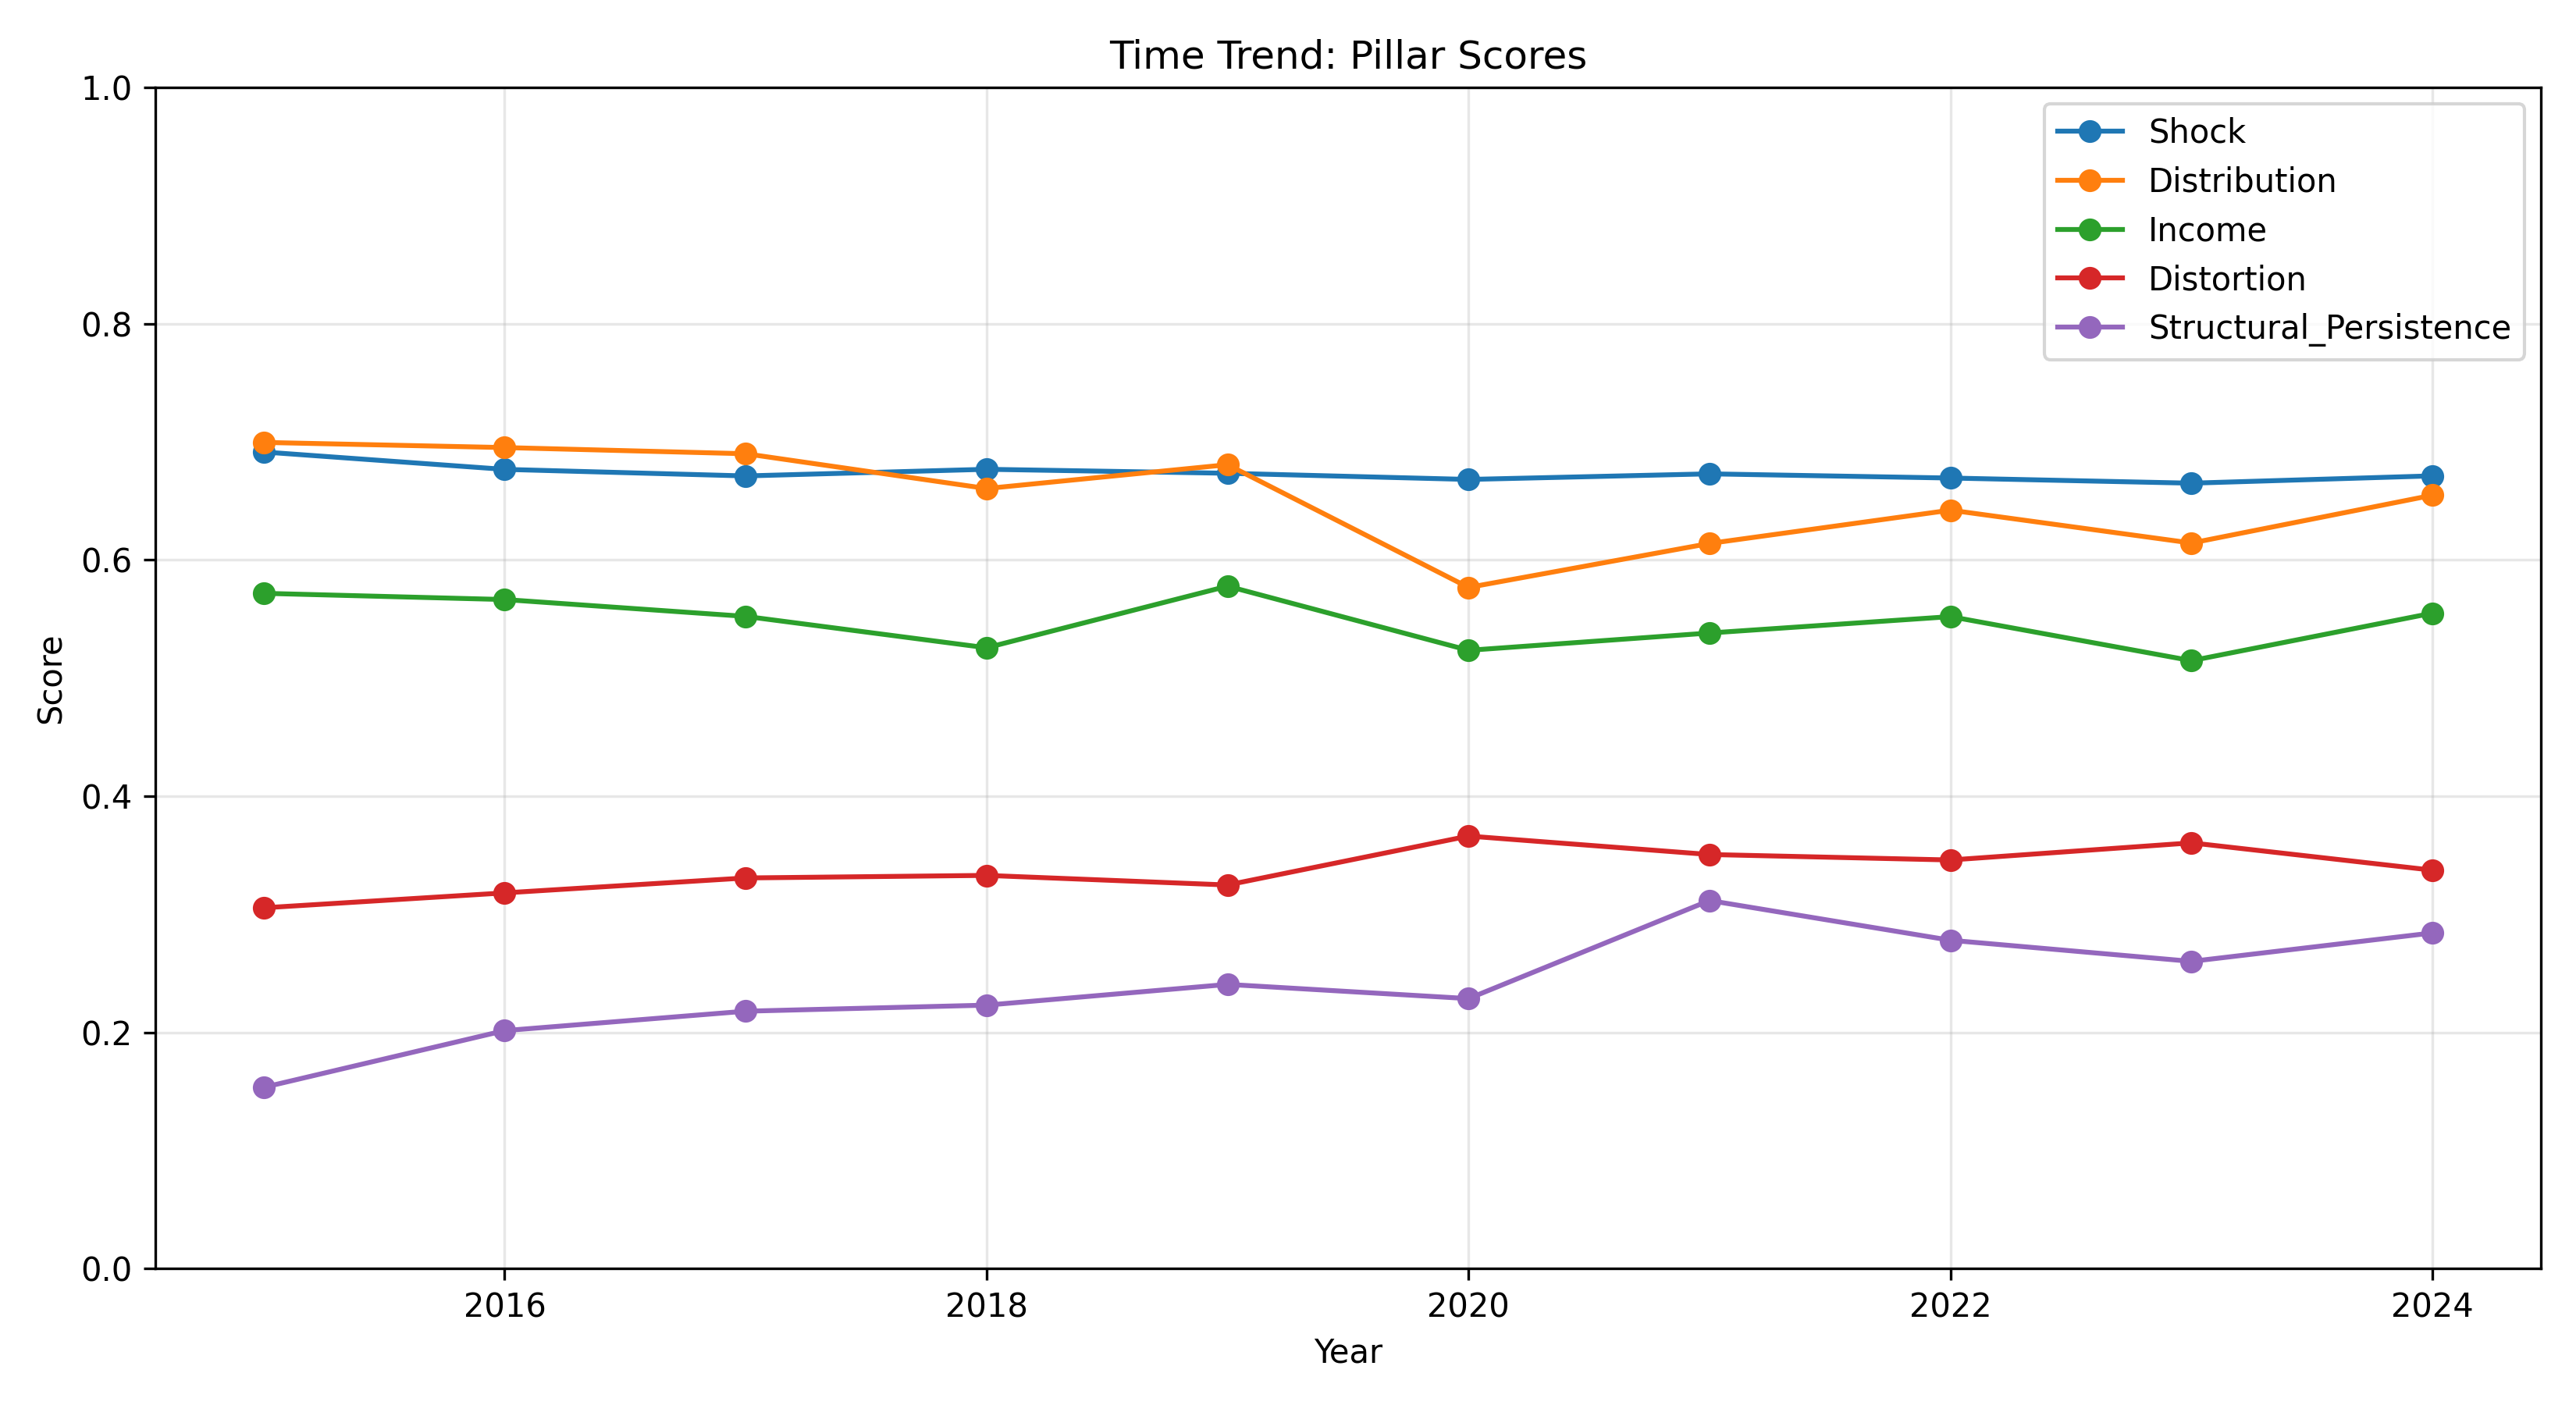
\includegraphics[width=0.9\textwidth]{figures/time_trend.png}
\caption{Time trends of composite index and individual pillars (2014–2024).}
\label{fig:time_trend}
\end{figure}

Figure \ref{fig:time_trend} shows the evolution of the composite index along with the five pillars over time. The overall index remains relatively stable across the period, indicating that MGNREGA provides consistent support rather than large fluctuations in impact.

This stability suggests that MGNREGA operates as a smoothing mechanism rather than a growth-enhancing intervention, with limited volatility in aggregate impact over time.

However, individual pillars display noticeable variation. During the COVID-19 period, a clear shift can be observed. Shock absorption remains strong, while income and distribution show a slight decline. At the same time, distortion increases, suggesting a change in the nature of the program.

These patterns indicate that MGNREGA is dynamic in its functioning and responds to broader economic conditions rather than operating as a static policy.

\subsection{Multi-Dimensional Performance: Radar Analysis}

\begin{figure}[H]
\centering

\includegraphics[width=0.7\textwidth]{figures/radar_post_covid.png}
\caption{Radar chart showing performance across five pillars (Post-COVID average).}
\label{fig:radar}
\end{figure}

Figure \ref{fig:radar} provides a summary of MGNREGA’s performance across all five dimensions. The program performs strongly in shock absorption, indicating its effectiveness as a safety net.

The radar representation allows for simultaneous comparison across dimensions, highlighting imbalances that would not be visible in univariate analysis.

The income and distribution pillars show moderate performance, suggesting that while welfare gains exist, they are not uniformly strong across all districts. Distortion appears relatively higher, indicating potential trade-offs between income support and efficiency.

Structural persistence shows moderate values, suggesting that the effects of MGNREGA extend beyond the immediate period but are not strong enough to indicate deep structural transformation.

Overall, the radar chart highlights that MGNREGA performs unevenly across dimensions, reinforcing the need for a multi-dimensional evaluation.

\subsection{Spatial Variation in Program Performance}

\begin{figure}[H]
\centering
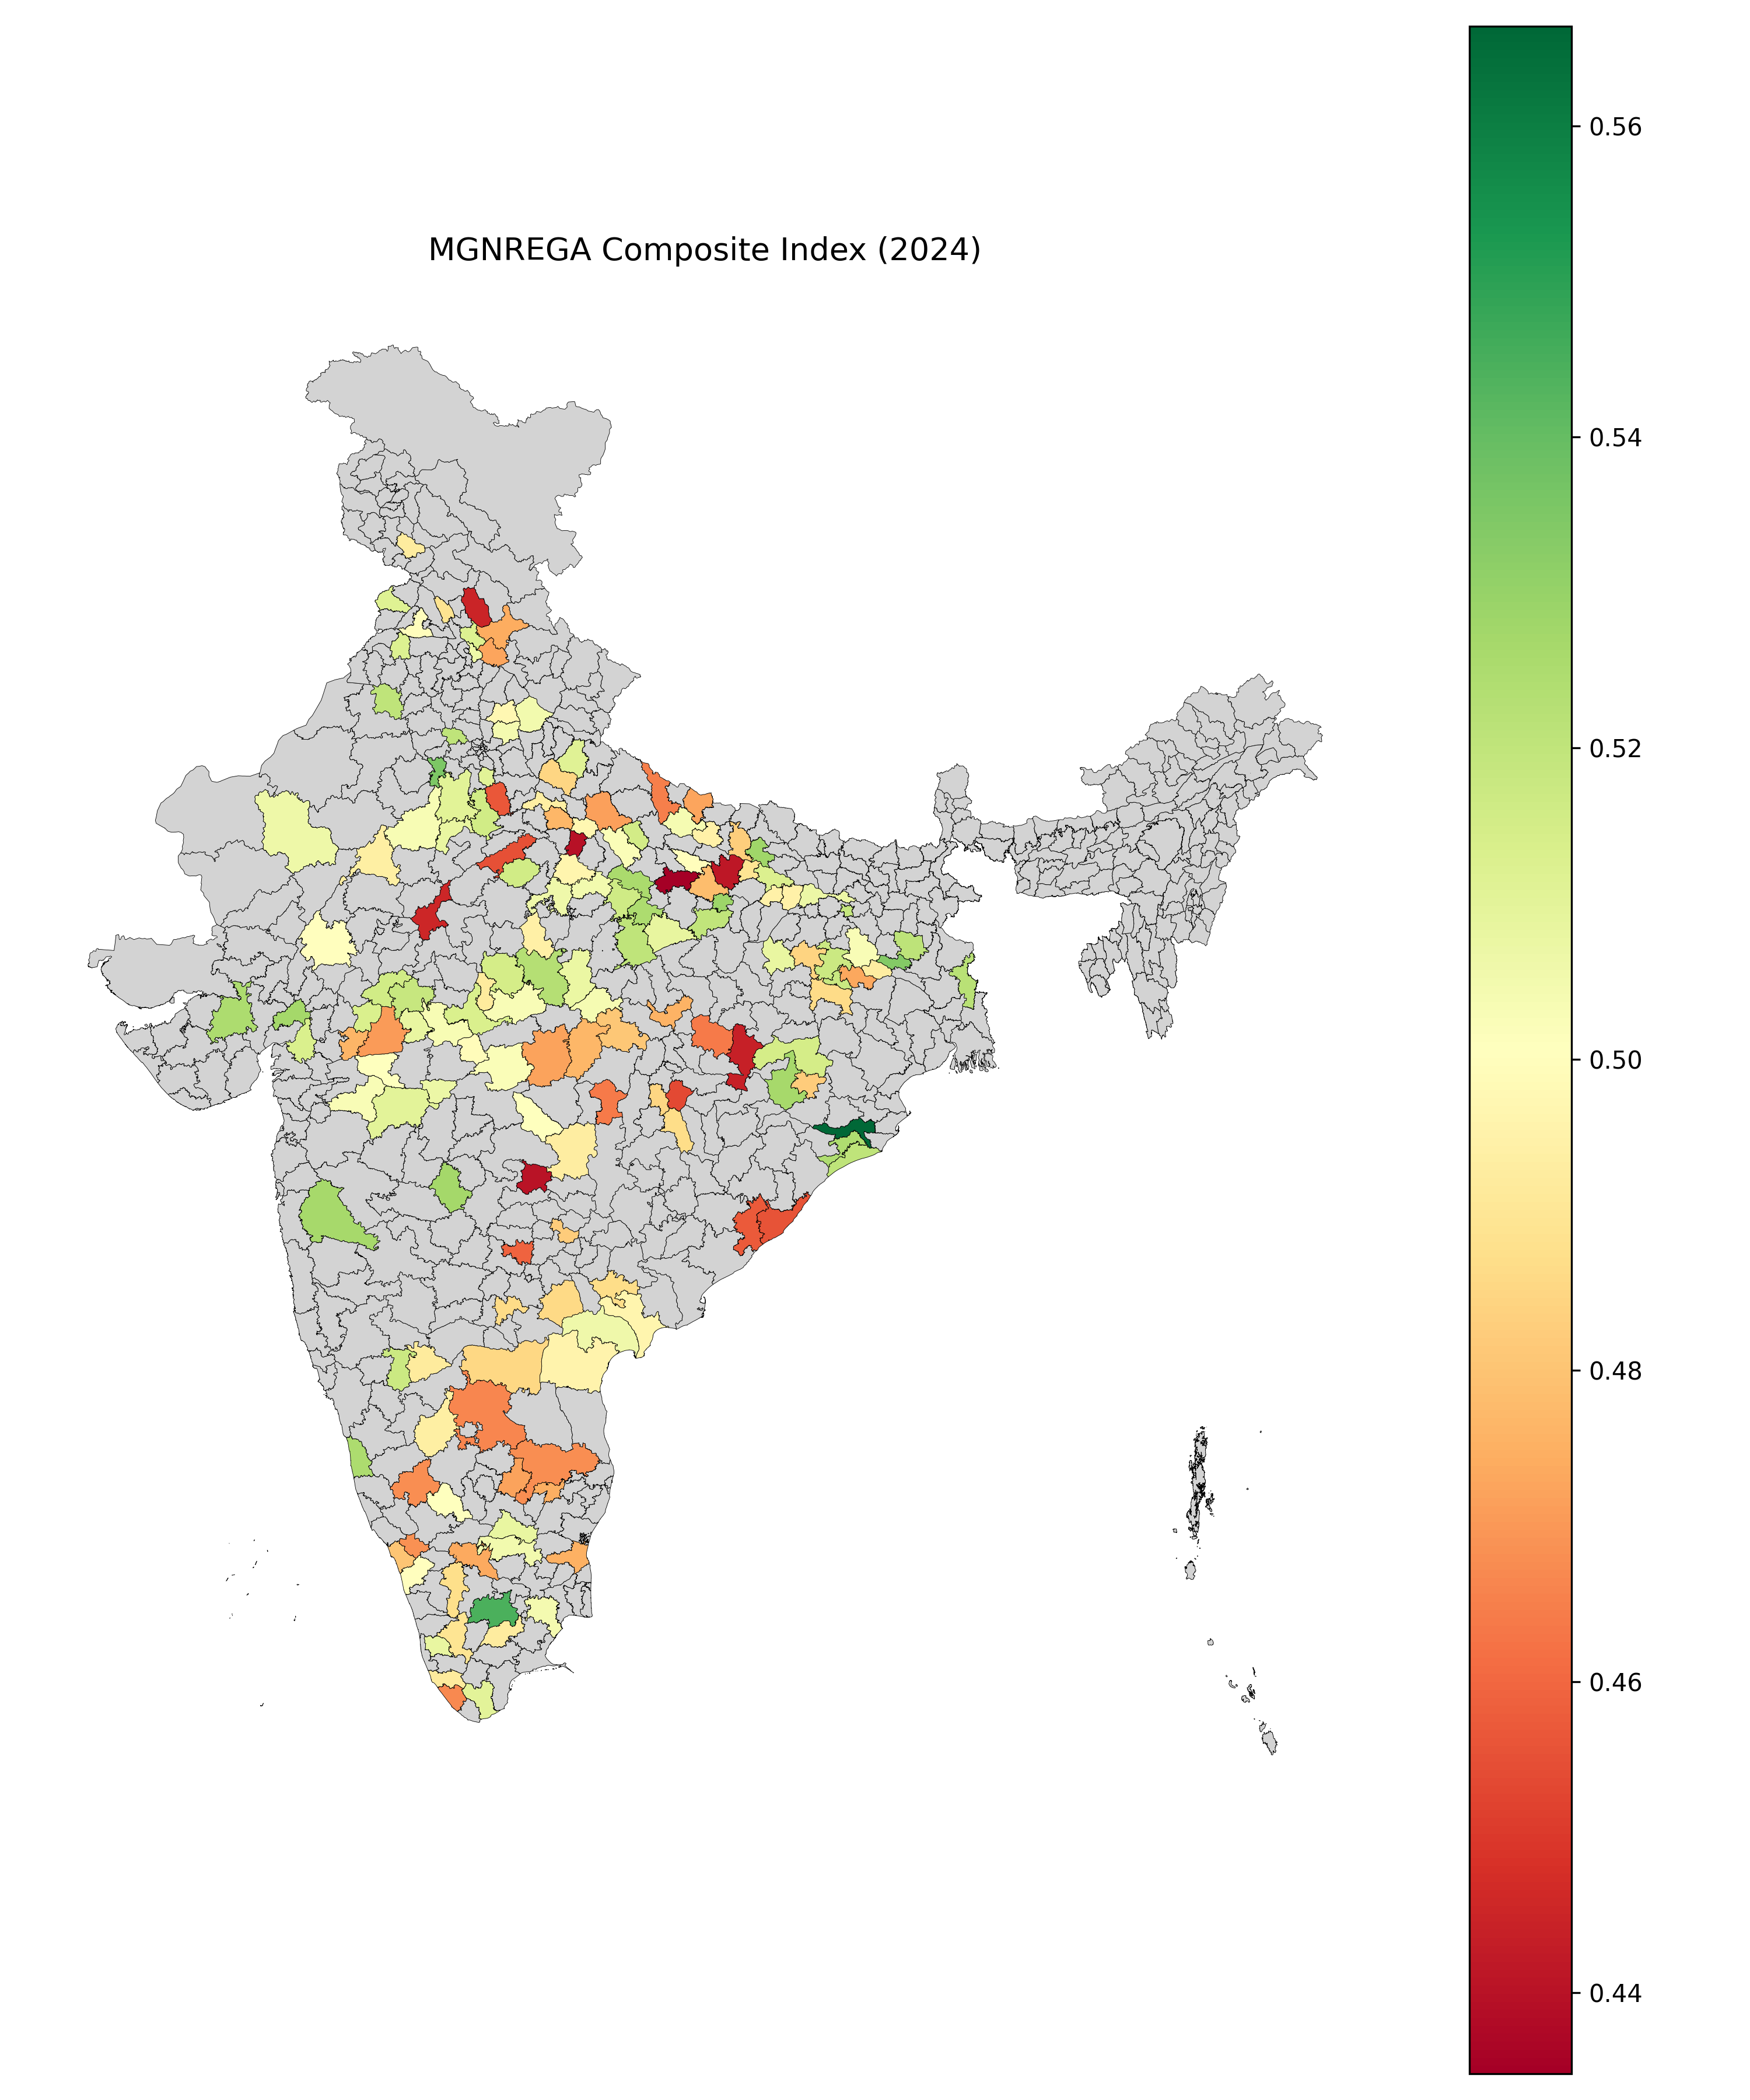
\includegraphics[width=0.85\textwidth]{figures/india_composite_map_2024.png}
\caption{District-level composite index of MGNREGA performance (2024).}
\label{fig:composite_map}
\end{figure}

Figure \ref{fig:composite_map} shows the spatial distribution of the composite index across districts. There is clear regional variation, with some districts consistently performing better than others.

This variation suggests that local factors—such as administrative capacity, economic conditions, and participation levels—play an important role in determining program outcomes.

\subsection{Pillar-wise Results}

\textbf{Shock Absorption:}
The results show that MGNREGA plays a strong role in stabilizing income during adverse conditions. The interaction estimates indicate that districts with higher program intensity experience smaller income losses during rainfall shocks.

\textbf{Distributional Effects:}
The distributional results show variation across districts, indicating that the benefits of MGNREGA are not evenly shared. While some regions display strong inclusion, others show weaker outcomes.

\textbf{Income Effects:}
The income pillar confirms that MGNREGA has a positive impact on district-level income. However, the magnitude of the effect remains moderate.

\textbf{Labor Market Distortion:}
The distortion results indicate variation in efficiency outcomes. In some districts, income gains are not matched by improvements in productivity, suggesting trade-offs.

\textbf{Structural Persistence:}
The structural analysis shows that MGNREGA has some lagged effects on income, indicating persistence. However, the magnitude varies and does not point to strong long-term transformation.

\subsection{Impact of COVID-19}

A comparison of pre- and post-COVID periods reveals a shift in the functioning of MGNREGA. During the COVID period:

\begin{itemize}
\item Shock absorption remains strong
\item Income and distribution decline slightly
\item Distortion increases
\item Structural persistence improves modestly
\end{itemize}

These changes suggest that the program shifted from a development-oriented role to a stabilization mechanism during periods of economic stress.

\subsection{Heterogeneity Across Regions}

The heterogeneity analysis shows that lower-income districts tend to benefit slightly more in terms of the composite index. Similarly, districts with higher exposure to shocks rely more heavily on MGNREGA.

This indicates that the program plays a relatively stronger role in economically weaker and more vulnerable regions.

\subsection{Dynamic Effects}

The dynamic analysis shows that lagged effects of MGNREGA on income are statistically significant, indicating persistence. At the same time, lead effects are not significant, suggesting that the program responds to current conditions rather than anticipated changes.

\subsection{Summary}

The results show that MGNREGA performs well as a safety net and income-support mechanism, but less strongly as a driver of long-term structural change. Its impact varies across regions and involves trade-offs across different economic dimensions.



\section{Economic Interpretation and Policy Insights}

The results presented in the previous section highlight that MGNREGA operates through multiple economic channels, each with different implications. This section interprets these findings and discusses their broader policy relevance.

\subsection{MGNREGA as a Stabilization Mechanism}

The strongest and most consistent result across the analysis is the role of MGNREGA as a safety net. The program performs well in stabilizing income during adverse conditions, particularly during the COVID period.

This suggests that MGNREGA functions effectively as a counter-cyclical policy tool, providing short-term support during economic stress. In the absence of formal insurance mechanisms in rural areas, this role becomes particularly important.

\subsection{Trade-offs Between Welfare and Efficiency}

The presence of distortion highlights an important trade-off. While MGNREGA increases income, it may also affect labor allocation and productivity.

This does not necessarily imply that the program is inefficient. Instead, it reflects a common policy trade-off between providing income support and maintaining market efficiency. In contexts where households face income risk, such trade-offs may be acceptable or even necessary.

\subsection{Uneven Distributional Outcomes}

The variation in distributional scores suggests that the inclusiveness of MGNREGA depends on local implementation and participation.

In some districts, the program successfully reaches marginalized groups, while in others the benefits are less evenly distributed. This indicates that improving targeting and participation mechanisms could enhance the equity impact of the program.

\subsection{Limited Structural Transformation}

The results show that while MGNREGA has some persistence effects, it does not lead to strong long-term structural transformation.

This suggests that the program should not be viewed as a standalone development tool. Instead, it is better understood as a support mechanism that needs to be complemented by other policies focused on productivity, infrastructure, and skill development.

\subsection{Regional Variation and Policy Design}

The strong regional variation observed in the results highlights the importance of localized policy design. A uniform approach may not be effective across all districts.

Allowing for flexibility in implementation, based on local economic conditions, could improve overall program effectiveness.

\subsection{Implications for Policy}

The findings of this study suggest several policy implications:

\begin{itemize}
\item Strengthen MGNREGA’s role as a safety net during economic shocks
\item Improve targeting to enhance distributional outcomes
\item Monitor and manage potential labor market distortions
\item Complement MGNREGA with long-term development policies
\item Encourage region-specific implementation strategies
\end{itemize}

Overall, MGNREGA should be viewed as a multi-purpose policy that balances welfare, equity, and stability, rather than as a single-outcome intervention.


\section{Conclusion}

This paper provides a multi-dimensional evaluation of MGNREGA using a district-level panel dataset spanning 2014–2024. Moving beyond traditional single-outcome analysis, we develop a five-pillar framework capturing shock absorption, distributional inclusion, income effects, labor market distortion, and structural persistence.

The results show that MGNREGA performs strongly as a stabilization mechanism, particularly during periods of economic stress such as the COVID-19 pandemic. The program is consistently associated with improved income outcomes and plays an important role in smoothing the effects of adverse shocks. However, its performance across other dimensions is more mixed. Distributional outcomes vary across districts, indicating uneven inclusion, while evidence of labor market distortion suggests trade-offs between welfare gains and efficiency.

At the same time, the analysis finds limited evidence of strong long-term structural transformation. While some persistence effects are observed, the magnitude remains modest, suggesting that MGNREGA primarily functions as a short-term support mechanism rather than a driver of sustained economic change.

A key contribution of this paper is the introduction of a unified framework that allows policy evaluation across multiple dimensions. This approach highlights that public policies such as MGNREGA cannot be fully understood through a single metric. Instead, they operate through multiple channels, often involving trade-offs between equity, efficiency, and stability.

The findings have important policy implications. Strengthening MGNREGA’s role as a safety net during economic shocks remains crucial, particularly in regions that are more vulnerable to income volatility. At the same time, improving targeting mechanisms can enhance distributional outcomes, while complementary policies focused on productivity and skill development are necessary to achieve long-term structural change.

Future research should focus on causal identification strategies and micro-level data to better isolate program impacts. Extending this framework to other large-scale welfare programs could further enhance its applicability in policy evaluation.


\newpage
\appendix

\section{Extended Exploratory Analysis}

This section presents additional exploratory analysis that complements the main findings discussed in Section 4. These figures provide deeper insights into regional variation, employment quality, and program dynamics.

\begin{figure}[H]
\centering
\IfFileExists{figures/state_level_comparison.png}{%
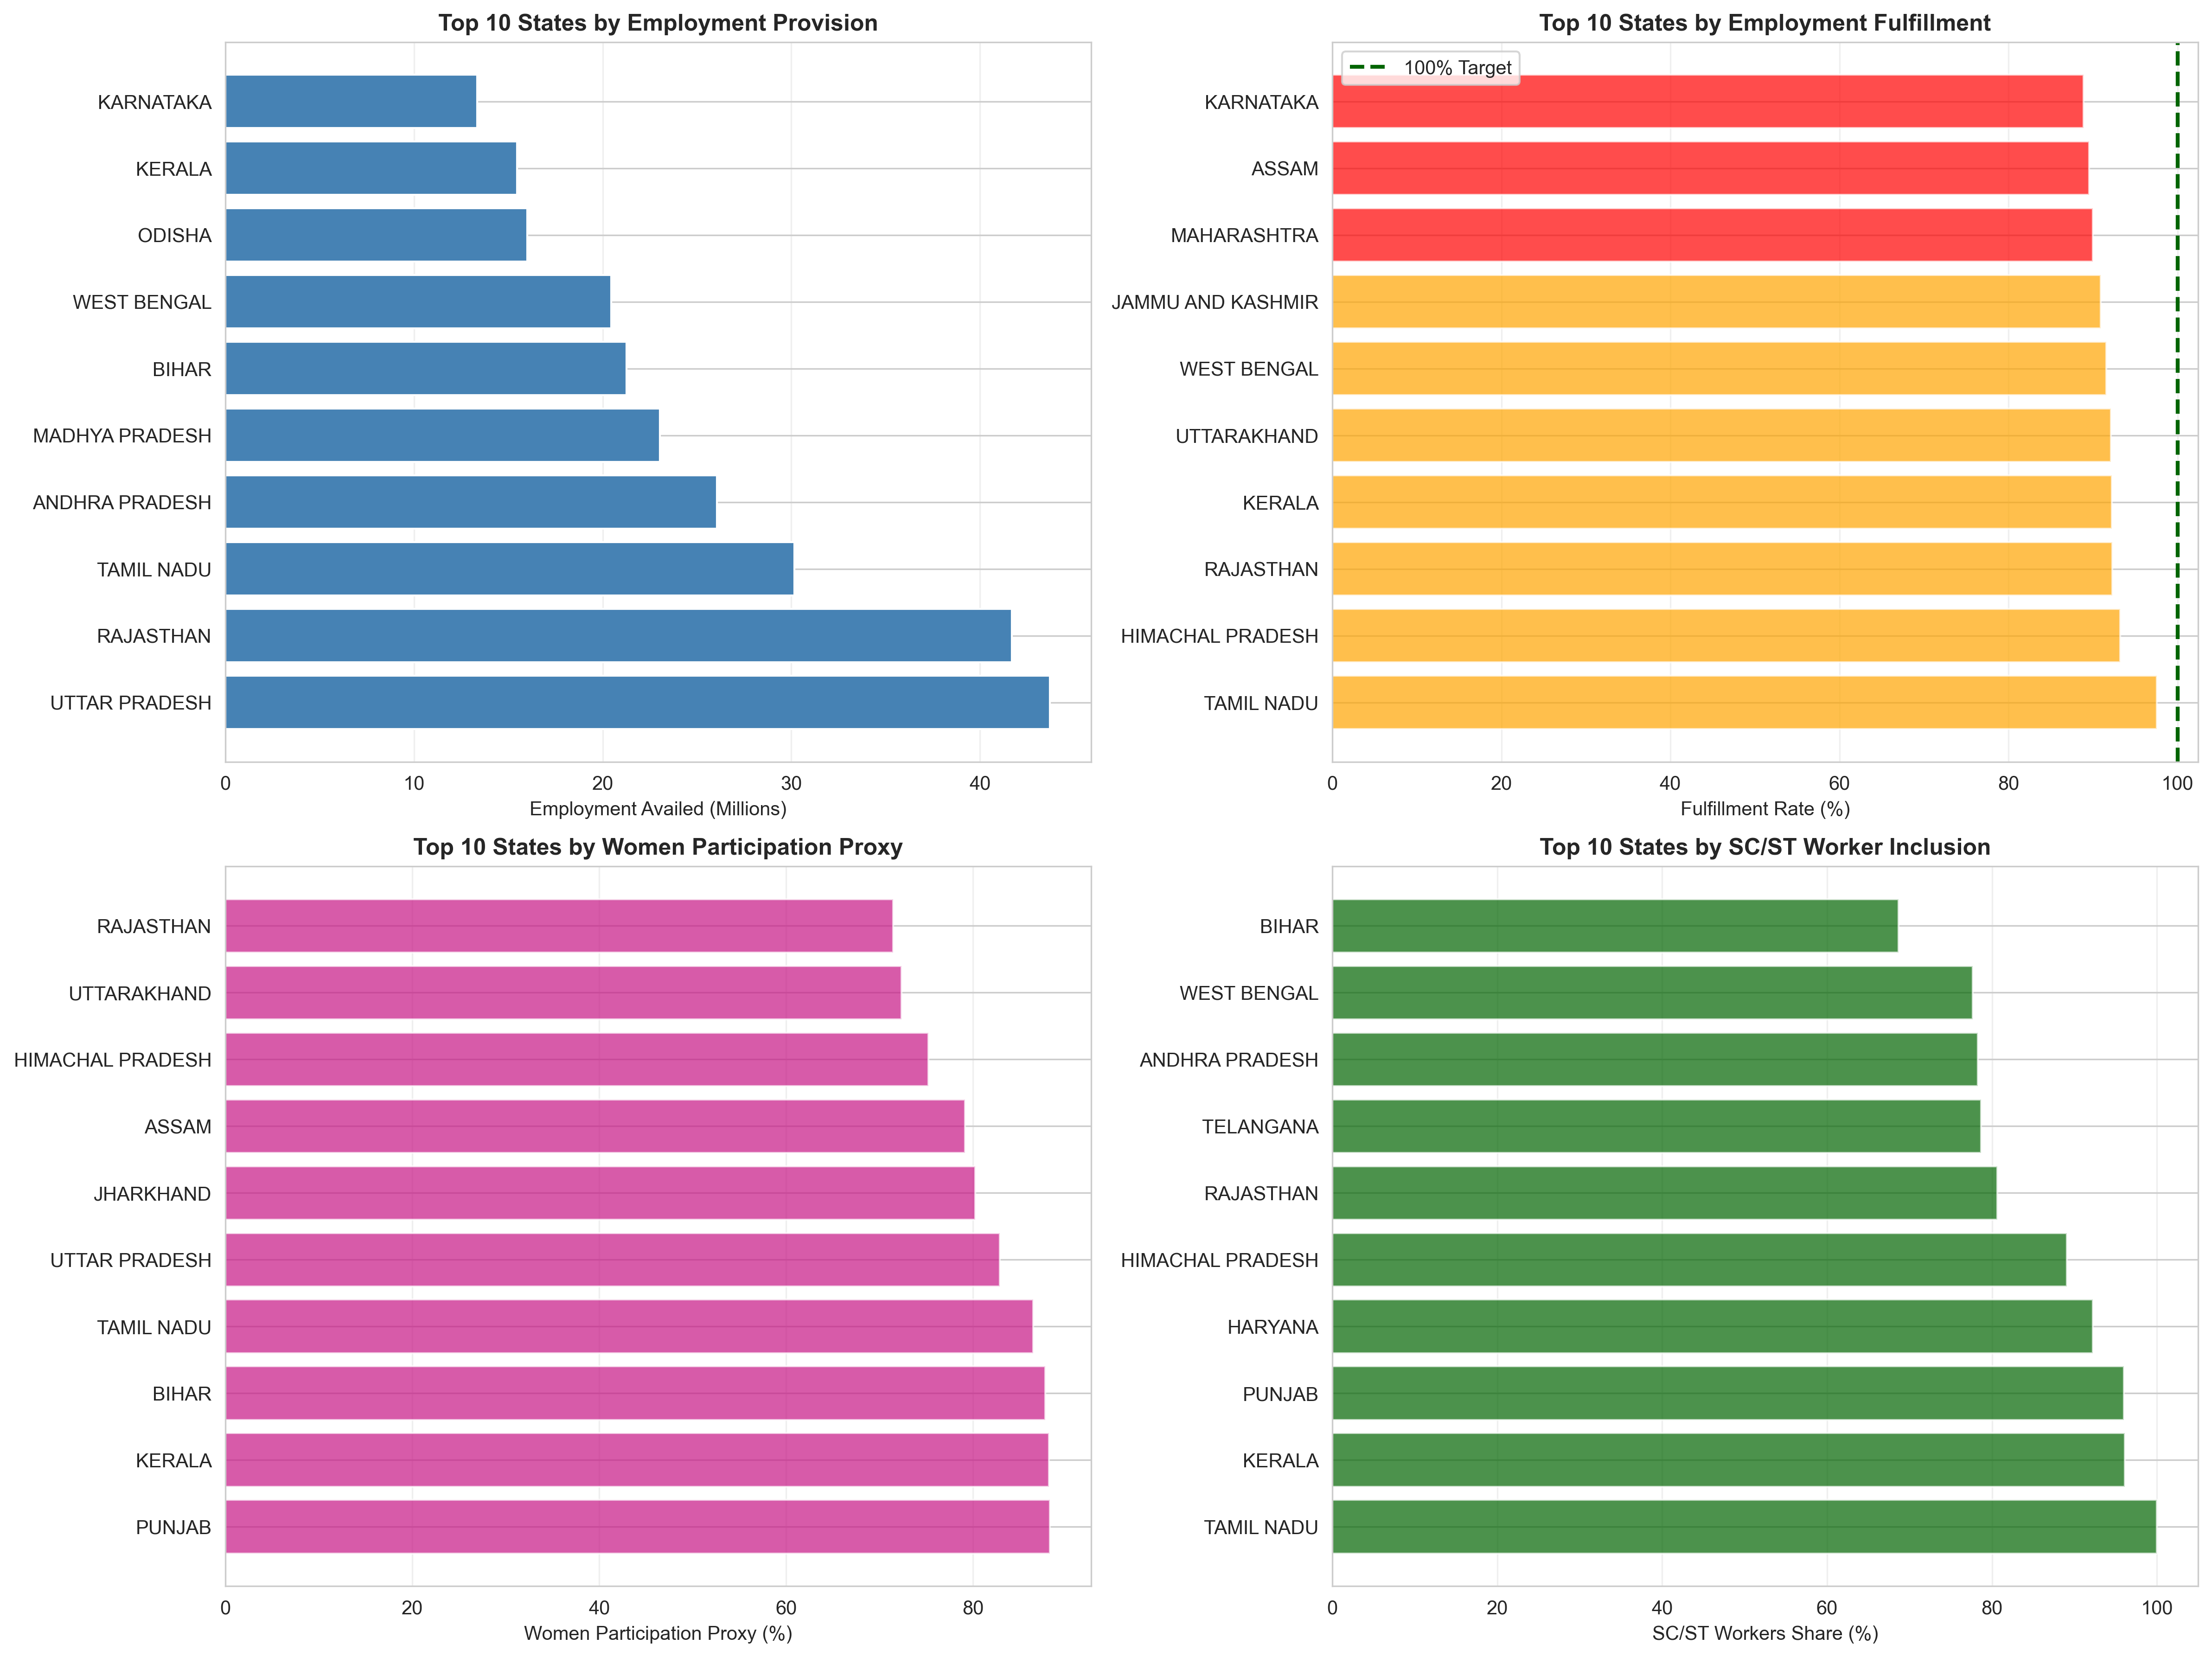
\includegraphics[width=0.9\textwidth]{figures/state_level_comparison.png}%
}{%
\fbox{\parbox[c][5cm][c]{0.85\textwidth}{\centering Missing figure: figures/state\_level\_comparison.png}}%
}
\caption{State-level comparison of MGNREGA performance indicators.}
\end{figure}

\begin{figure}[H]
\centering
\IfFileExists{figures/employment_quality.png}{%
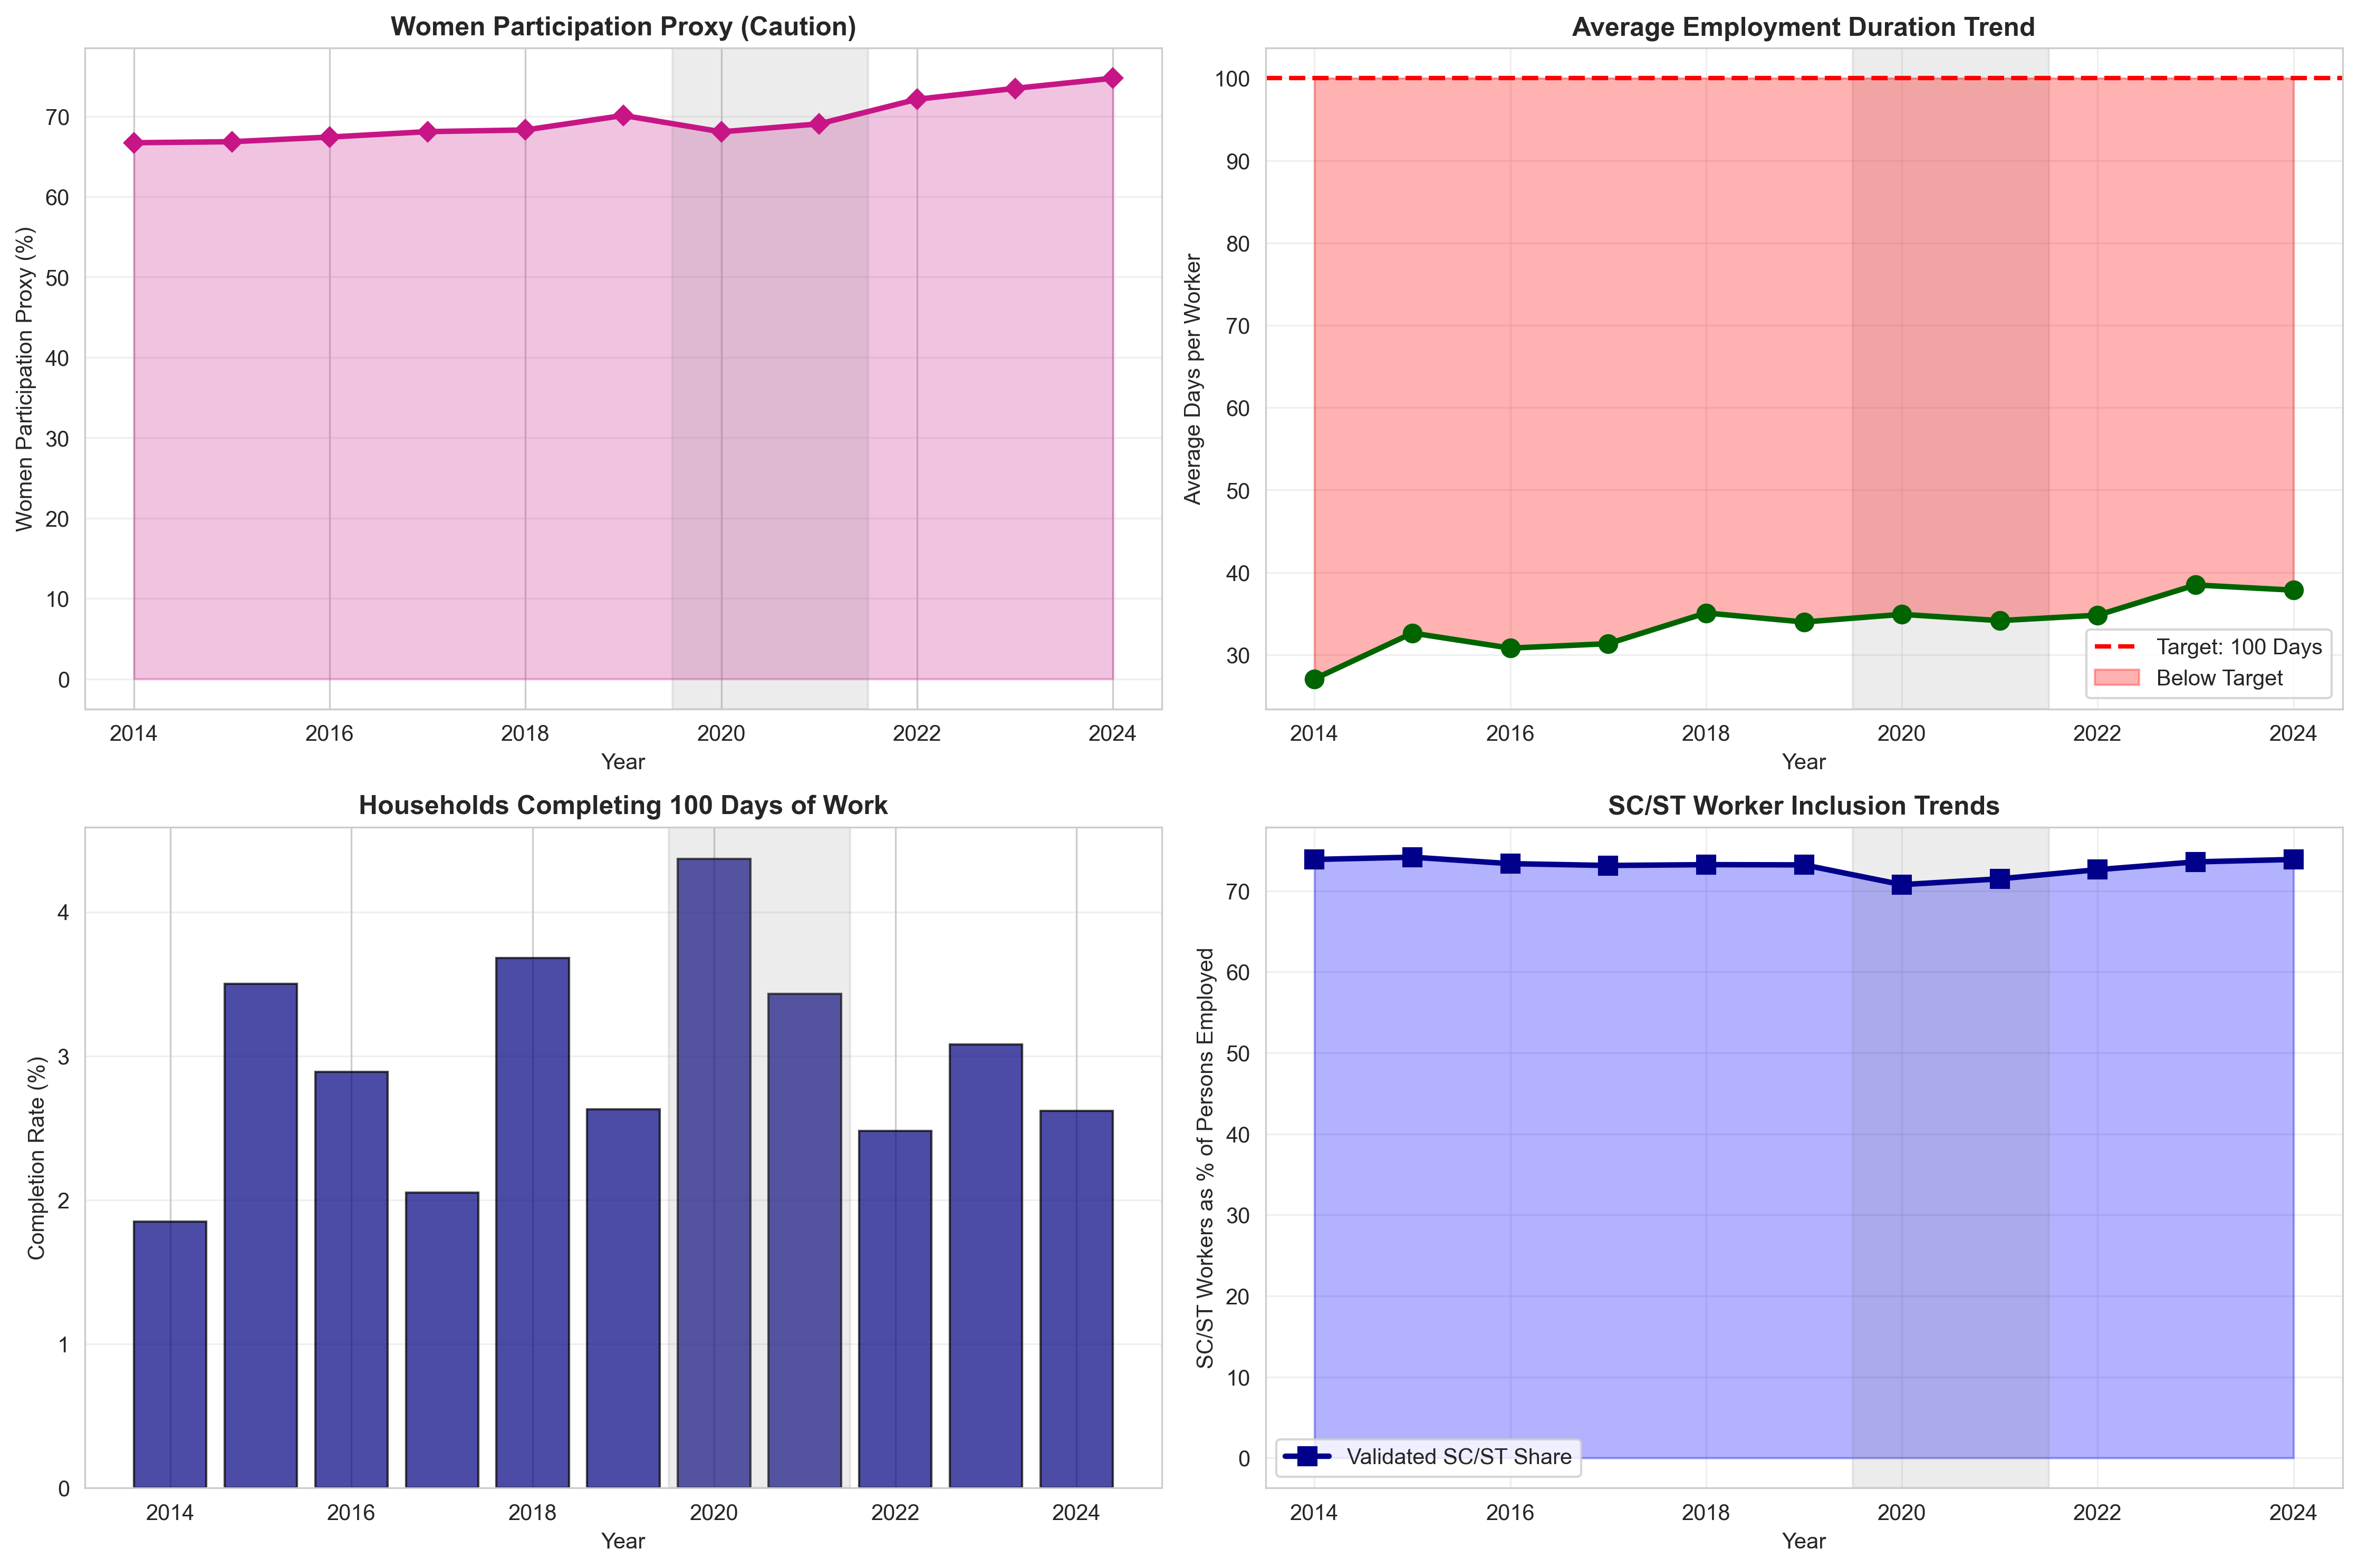
\includegraphics[width=0.9\textwidth]{figures/employment_quality.png}%
}{%
\fbox{\parbox[c][5cm][c]{0.85\textwidth}{\centering Missing figure: figures/employment\_quality.png}}%
}
\caption{Employment quality indicators including completion rates and participation patterns.}
\end{figure}

\begin{figure}[H]
\centering
\IfFileExists{figures/dashboard_summary.png}{%
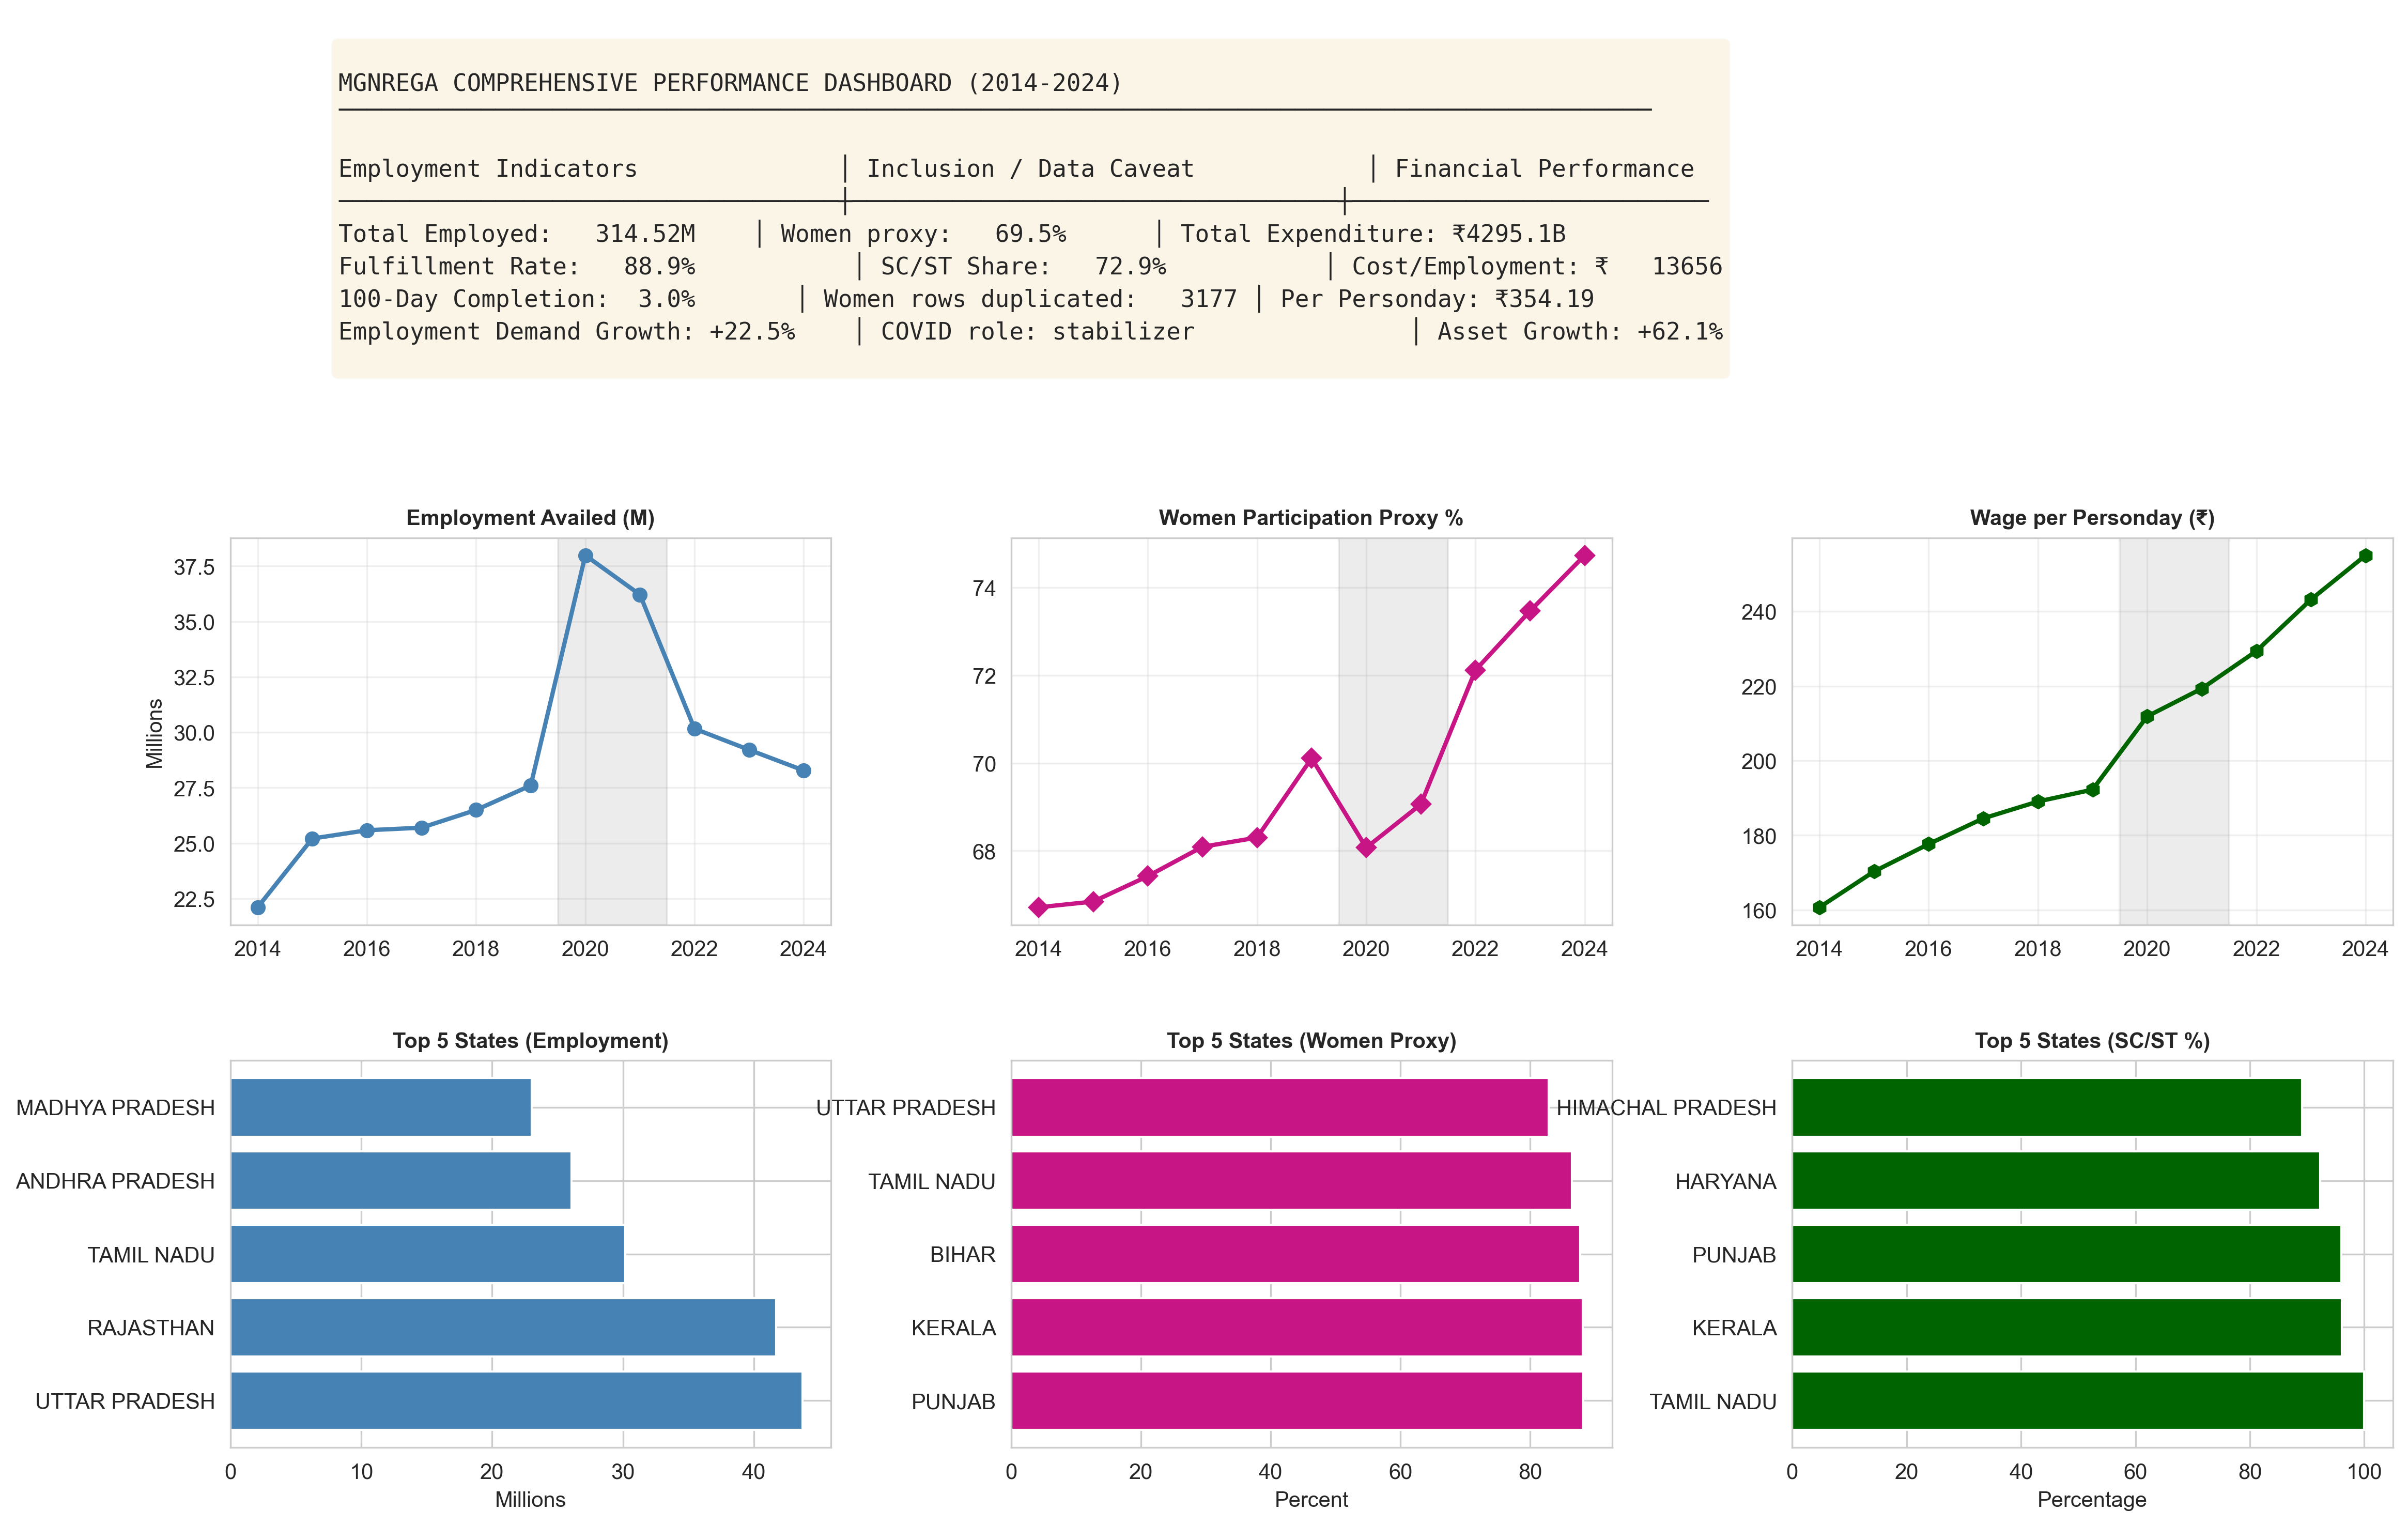
\includegraphics[width=0.9\textwidth]{figures/dashboard_summary.png}%
}{%
\fbox{\parbox[c][5cm][c]{0.85\textwidth}{\centering Missing figure: figures/dashboard\_summary.png}}%
}
\caption{Dashboard summary of key MGNREGA indicators.}
\end{figure}

These additional figures reinforce the presence of regional heterogeneity and variations in implementation quality across districts.


\section{MGNREGA Data Collection and Processing Pipeline}

The MGNREGA dataset used in this study is constructed through a custom web scraping pipeline that extracts district-level information from official government sources.

The pipeline involves the following steps:

\begin{itemize}
\item Automated extraction of district-level reports from official MGNREGA portals
\item Parsing of structured tables containing employment, wage, and participation data
\item Cleaning of inconsistent district names and formats
\item Handling of missing values through interpolation where appropriate
\item Aggregation of data to annual district-level observations
\end{itemize}

Special attention is given to ensuring consistency across years and districts. Duplicate entries are removed, and validation checks are performed to ensure data reliability.

This pipeline allows for the creation of a consistent and comprehensive dataset suitable for panel analysis.


\section{Additional Spatial Visualizations}

This section presents additional district-level maps for individual pillars that are not included in the main text.

\begin{figure}[H]
\centering
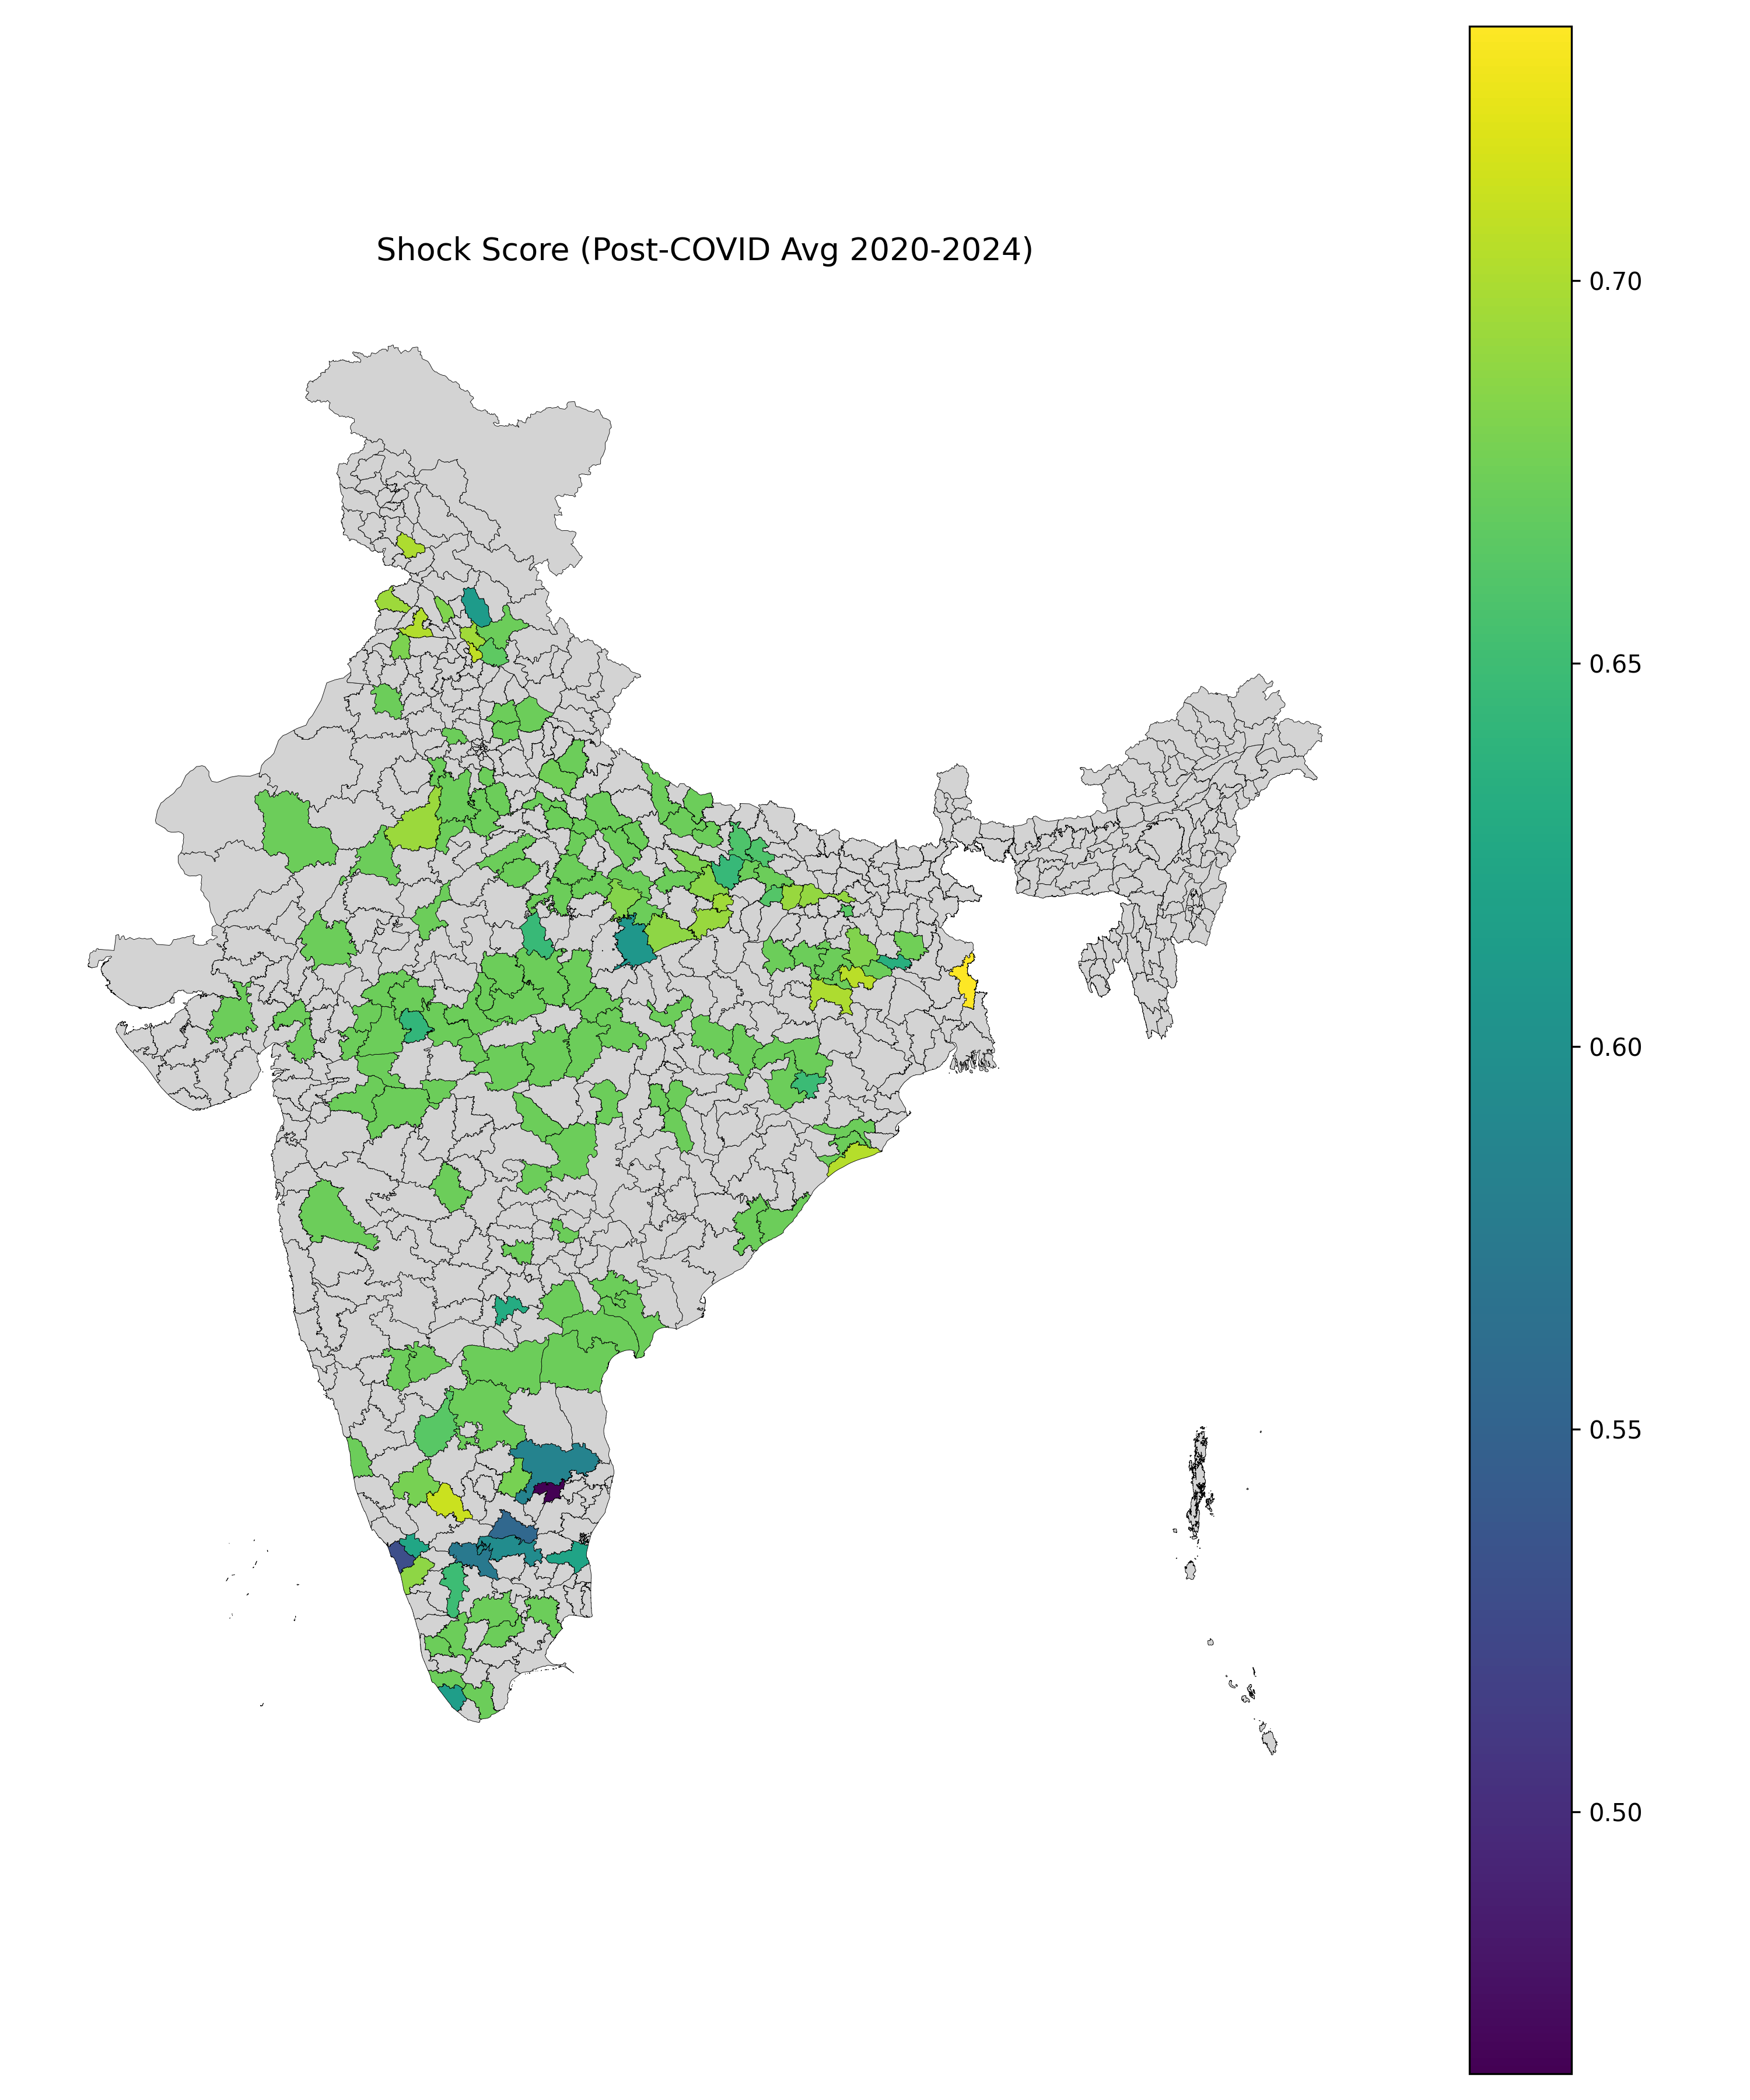
\includegraphics[width=0.85\textwidth]{figures/india_shock_map.png}
\caption{Shock absorption scores across districts.}
\end{figure}

\begin{figure}[H]
\centering
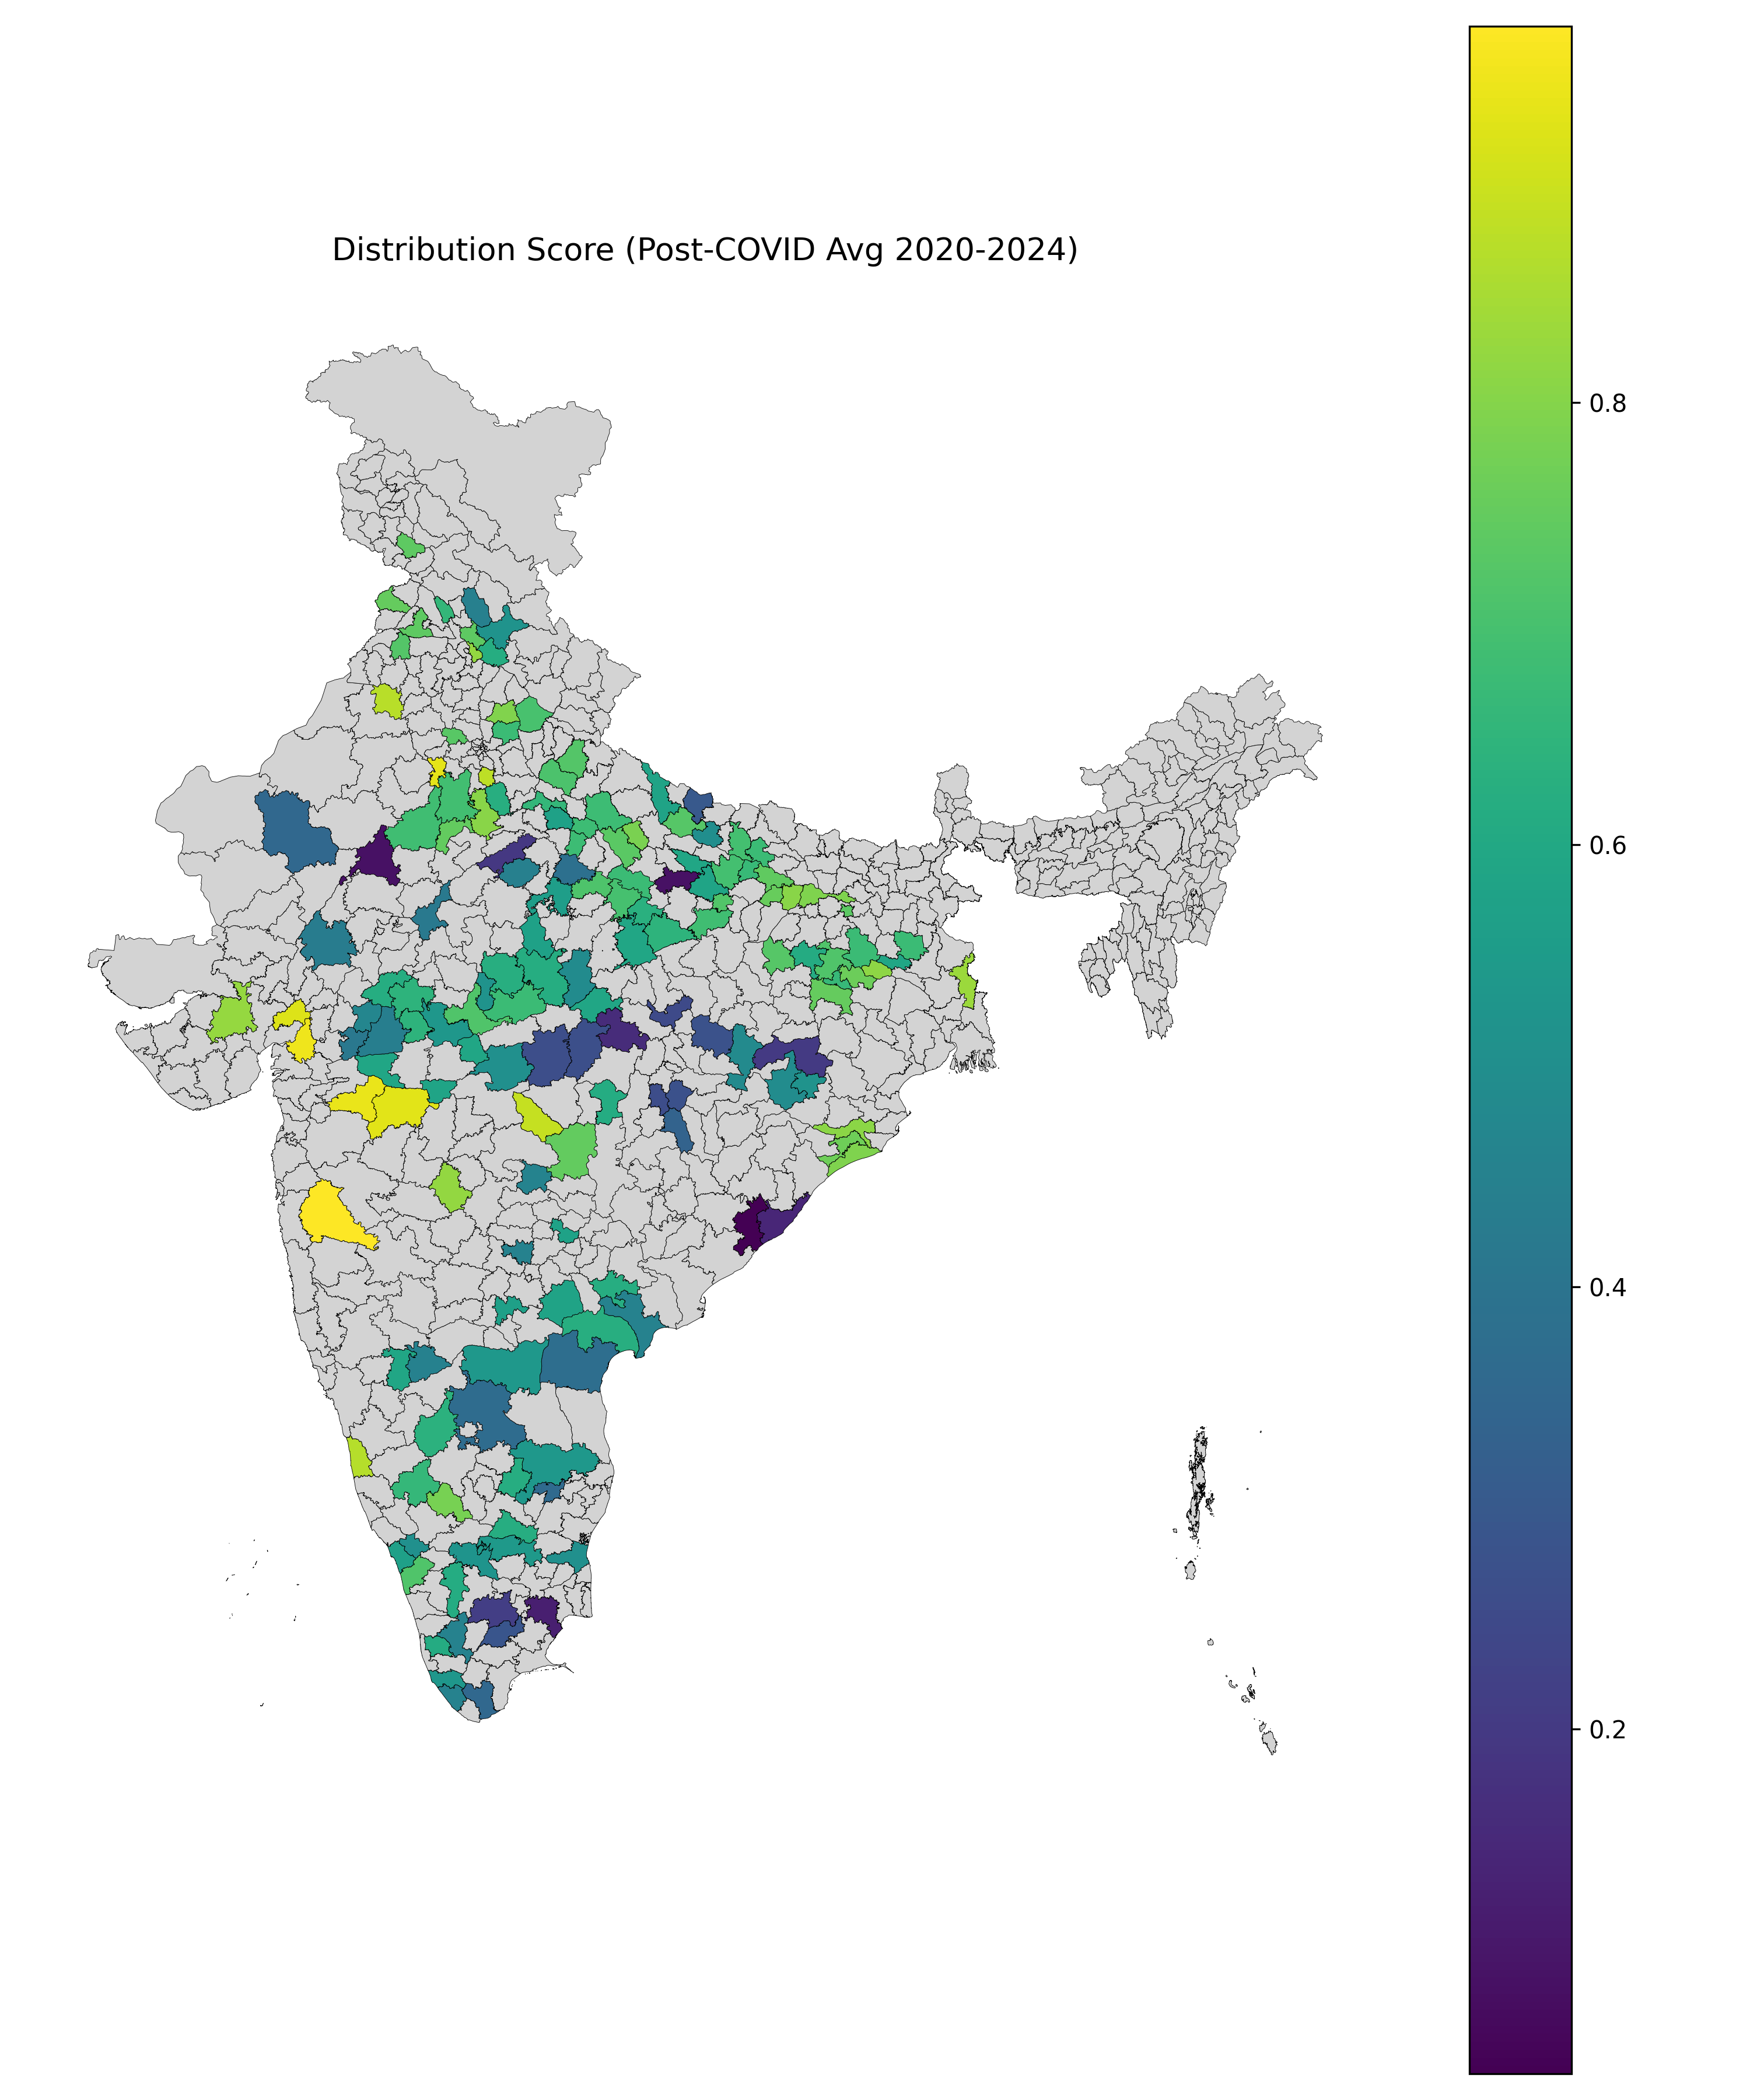
\includegraphics[width=0.85\textwidth]{figures/india_distribution_map.png}
\caption{Distributional scores across districts.}
\end{figure}

\begin{figure}[H]
\centering
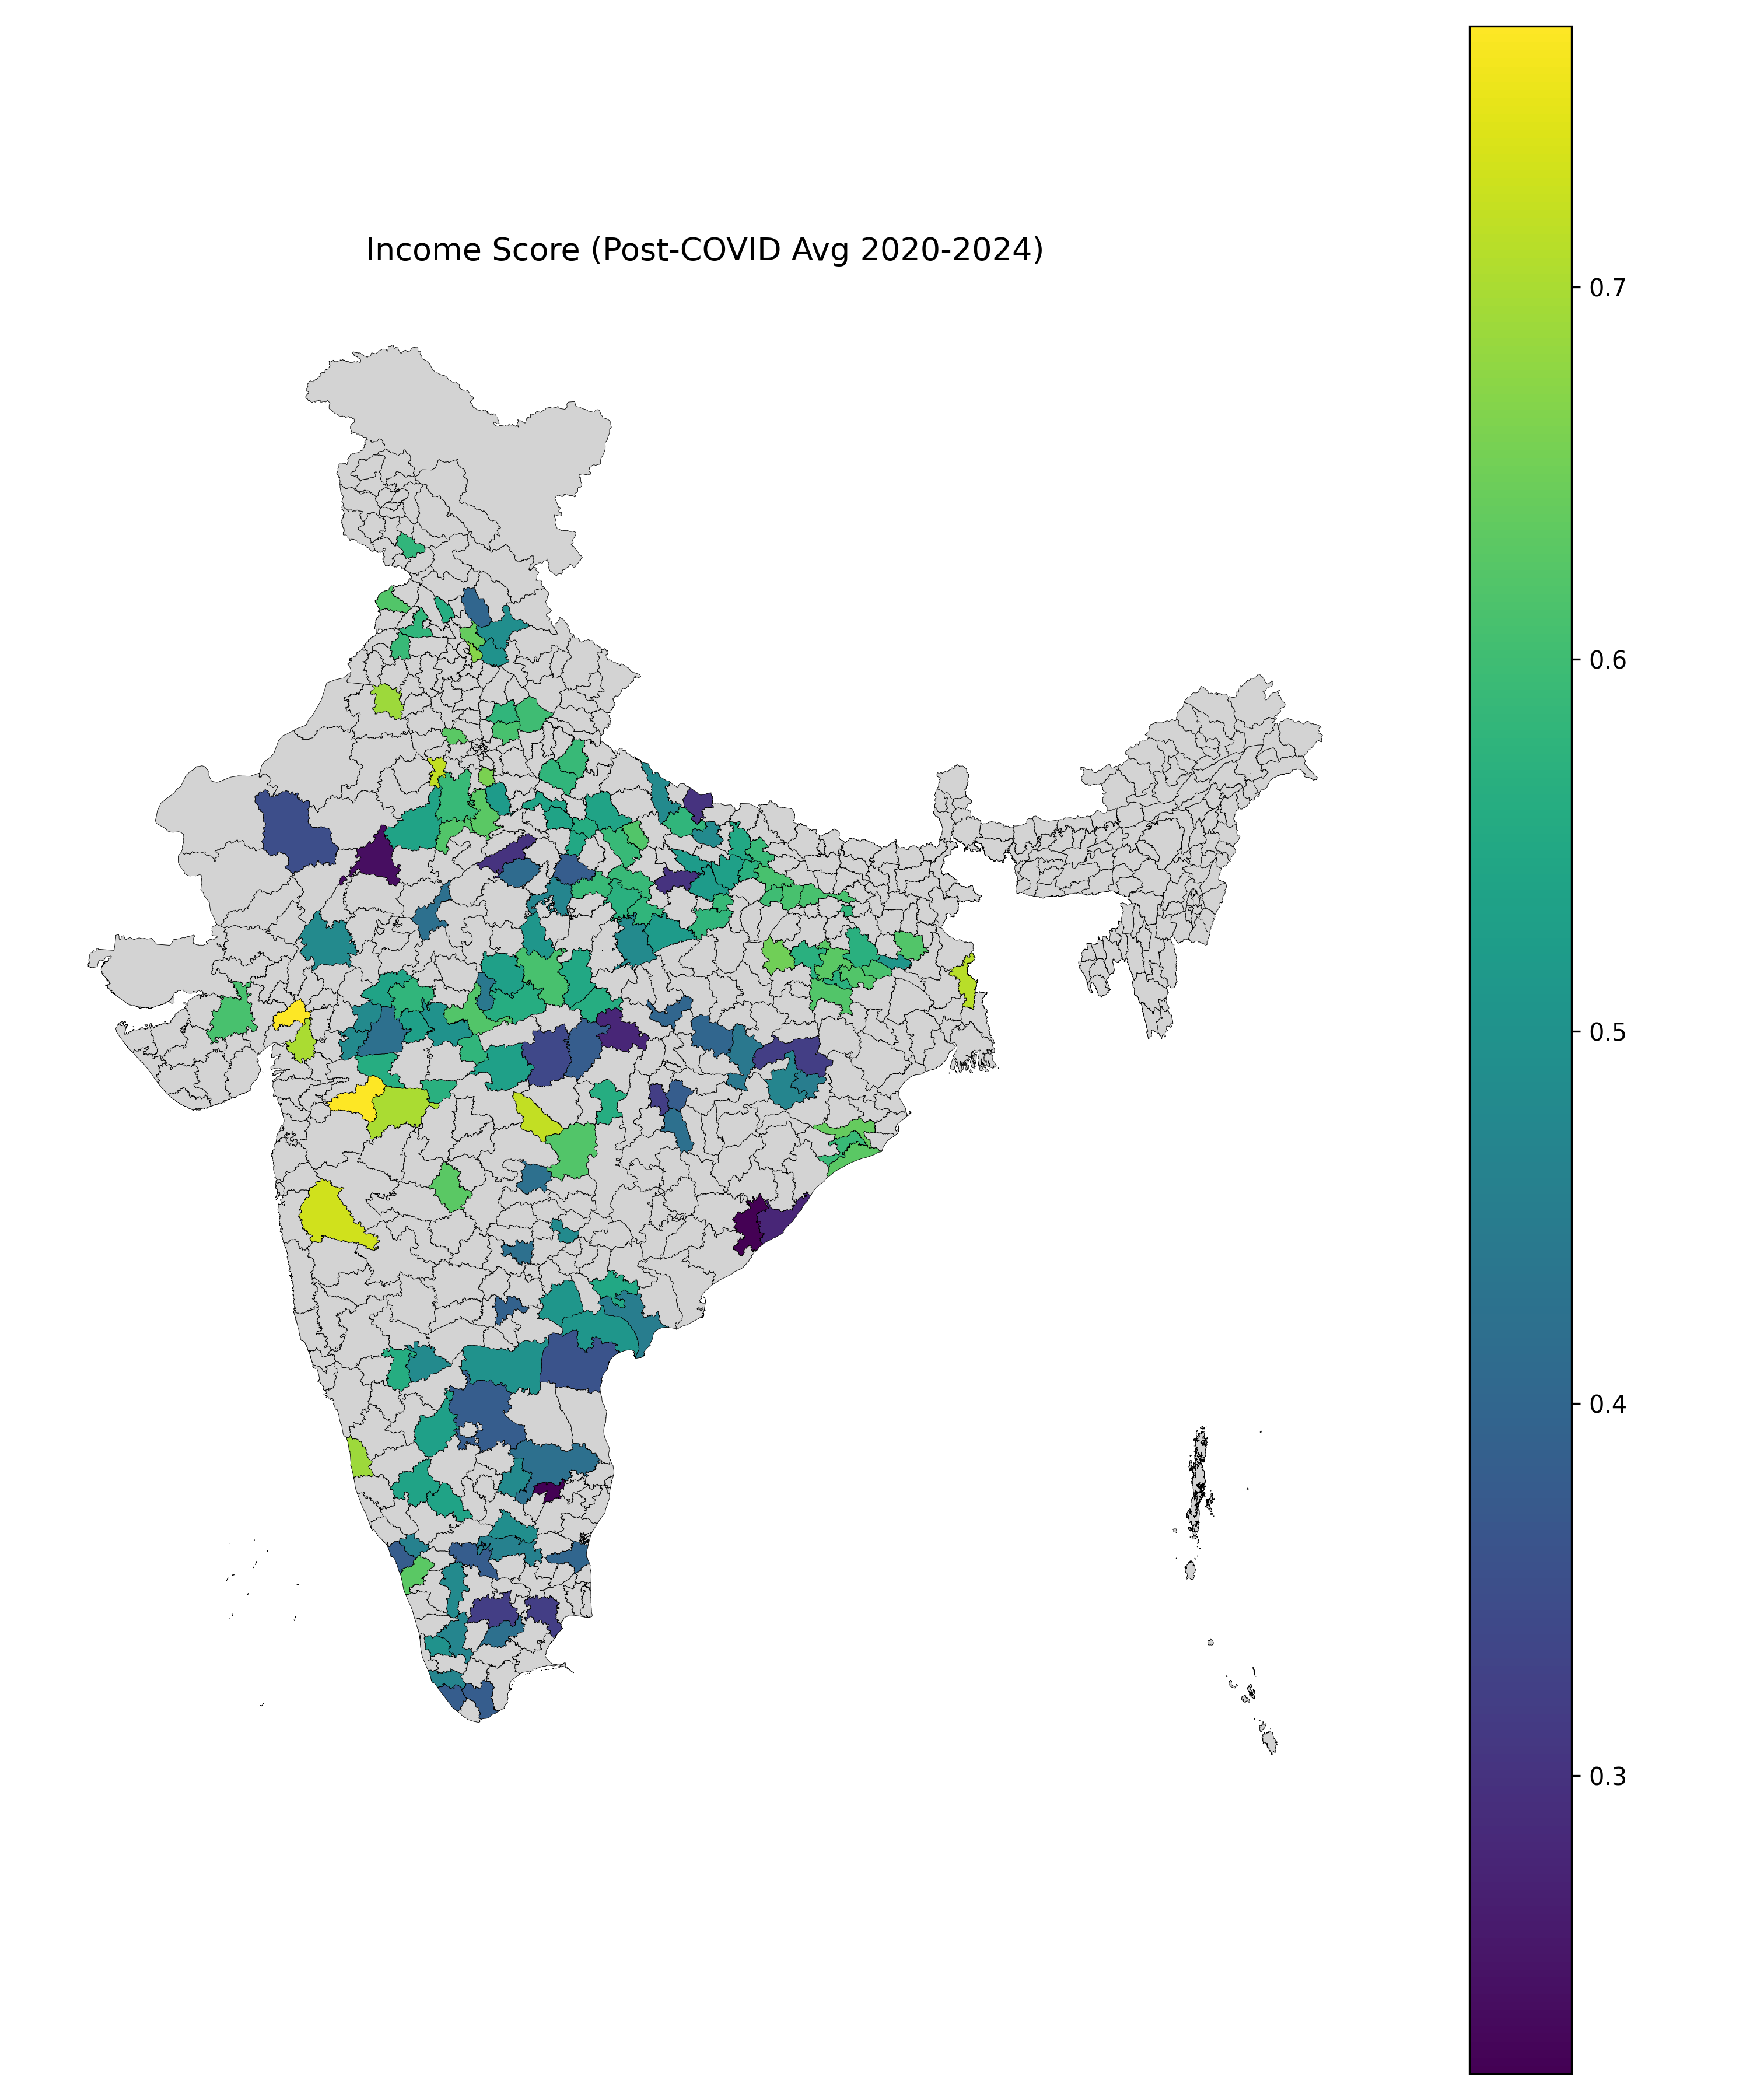
\includegraphics[width=0.85\textwidth]{figures/india_income_map.png}
\caption{Income scores across districts.}
\end{figure}

\begin{figure}[H]
\centering
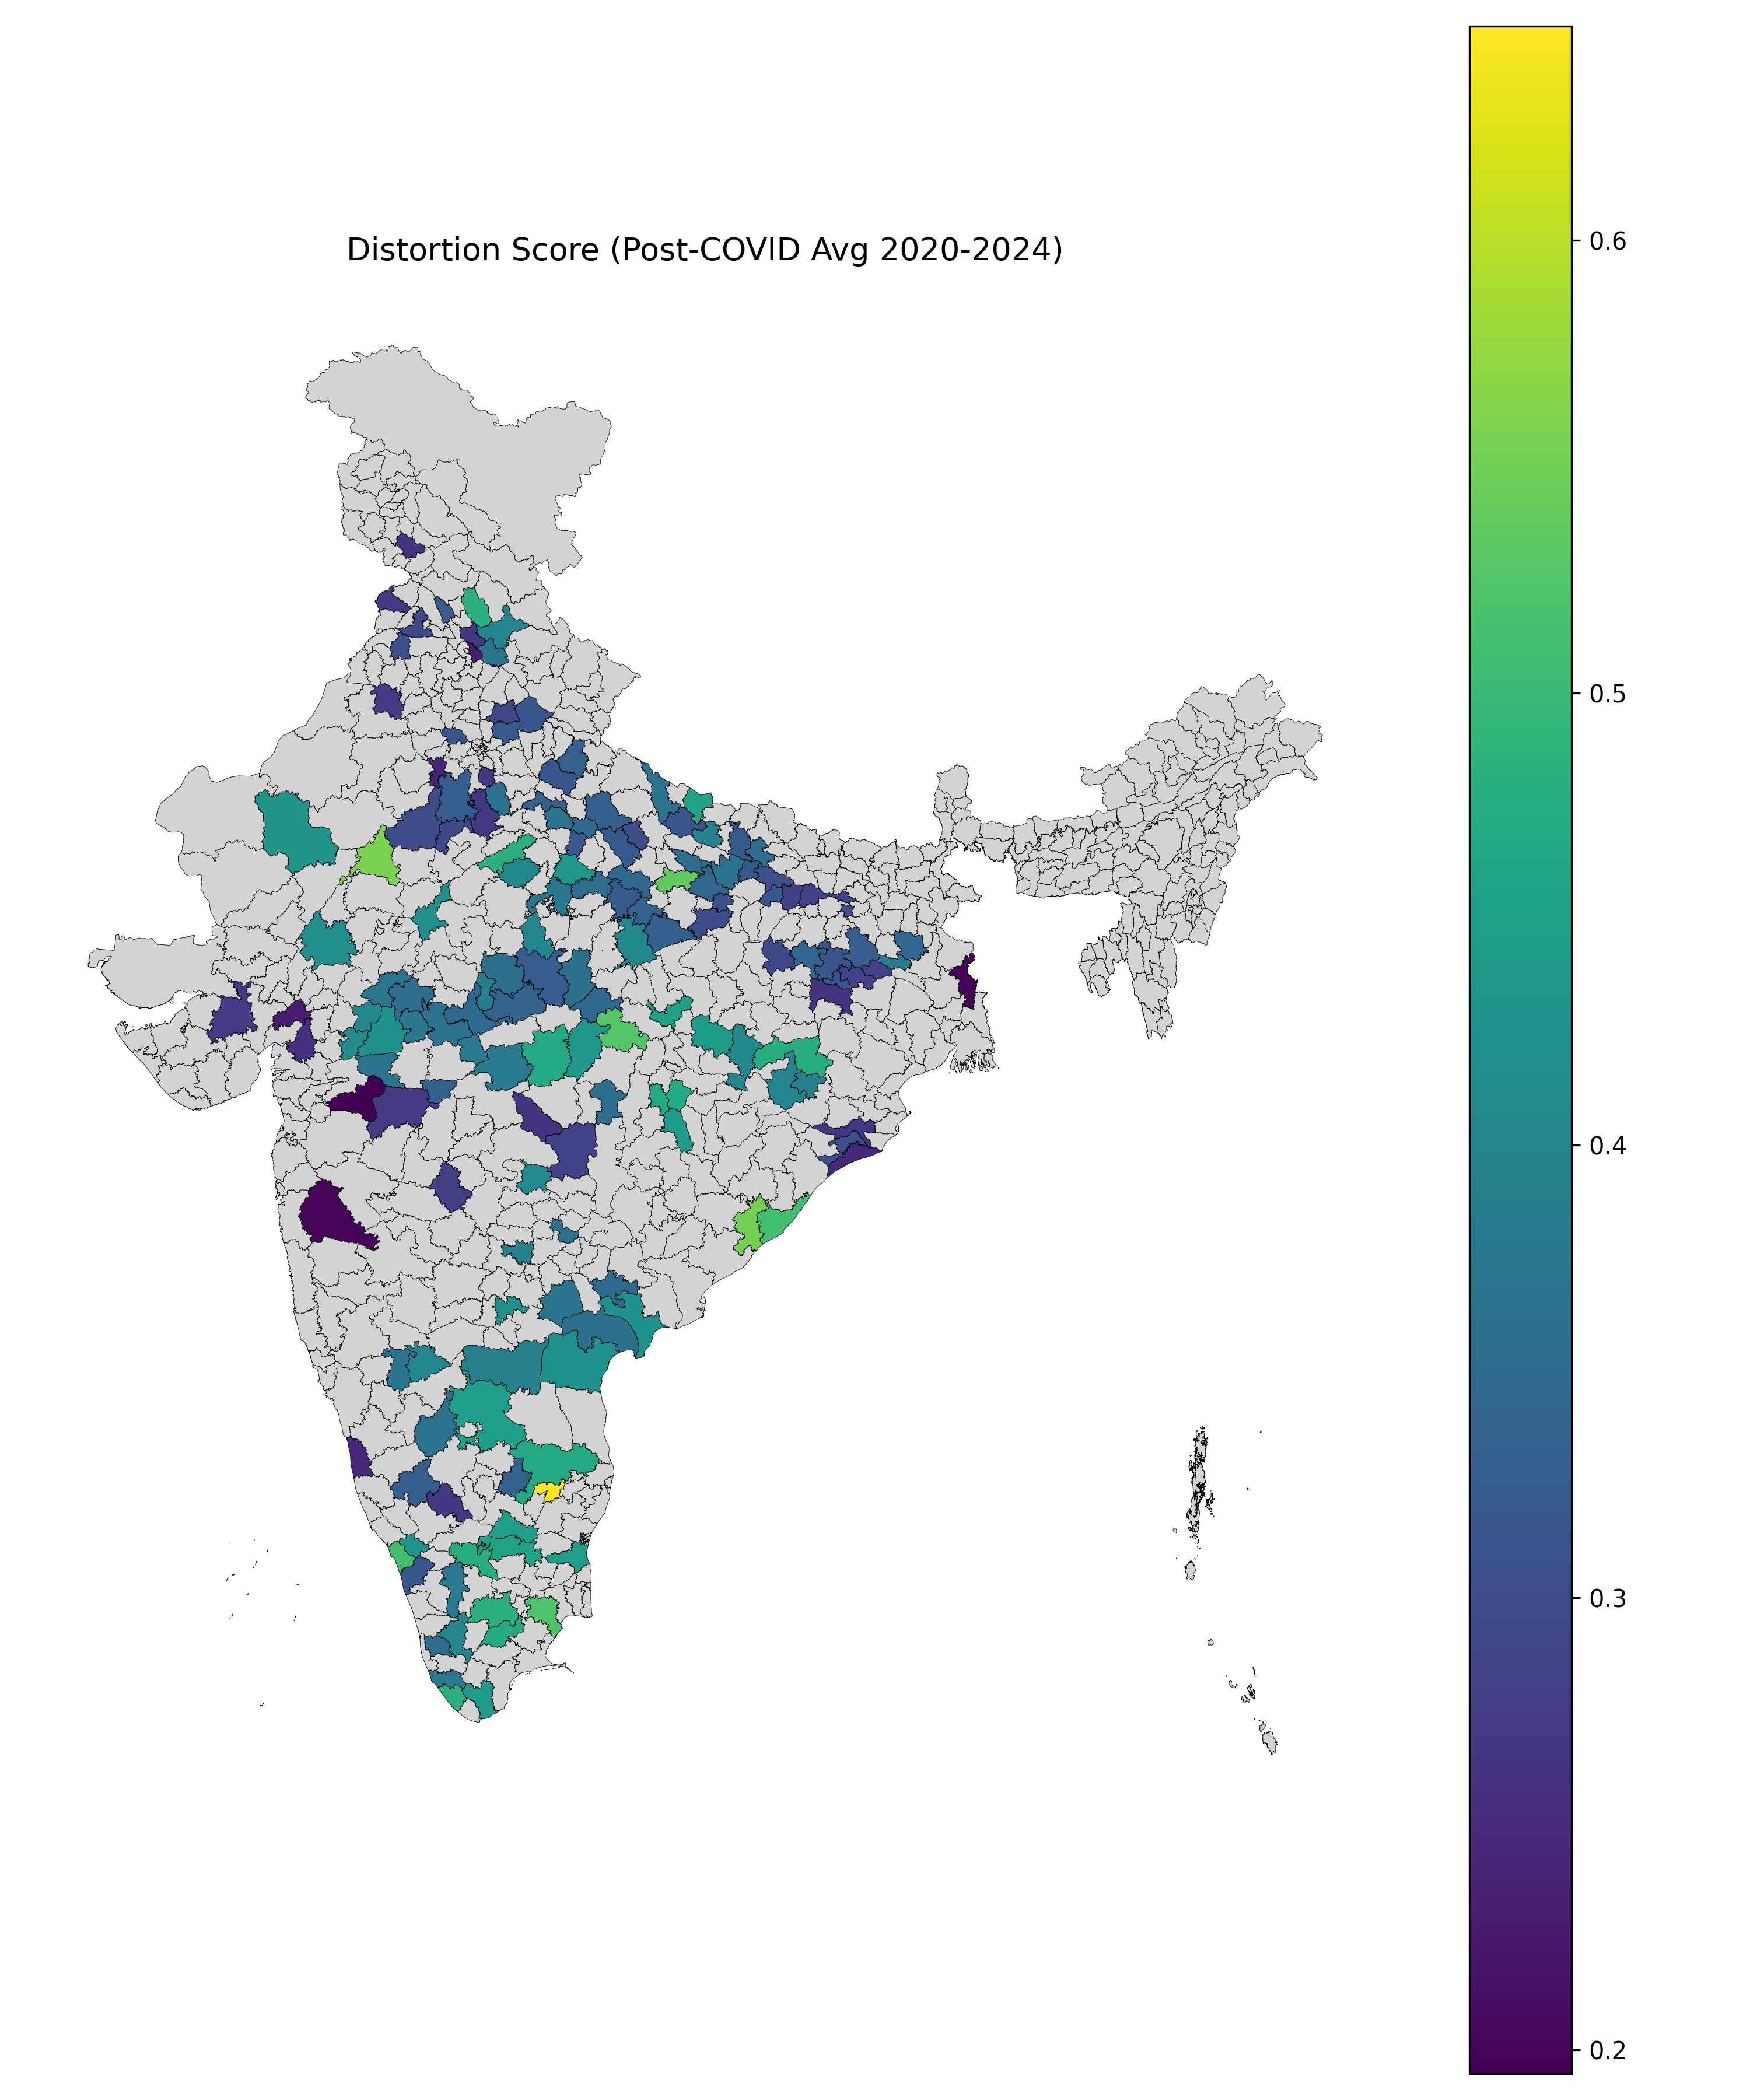
\includegraphics[width=0.85\textwidth]{figures/india_distortion_map.png}
\caption{Distortion scores across districts.}
\end{figure}

\begin{figure}[H]
\centering
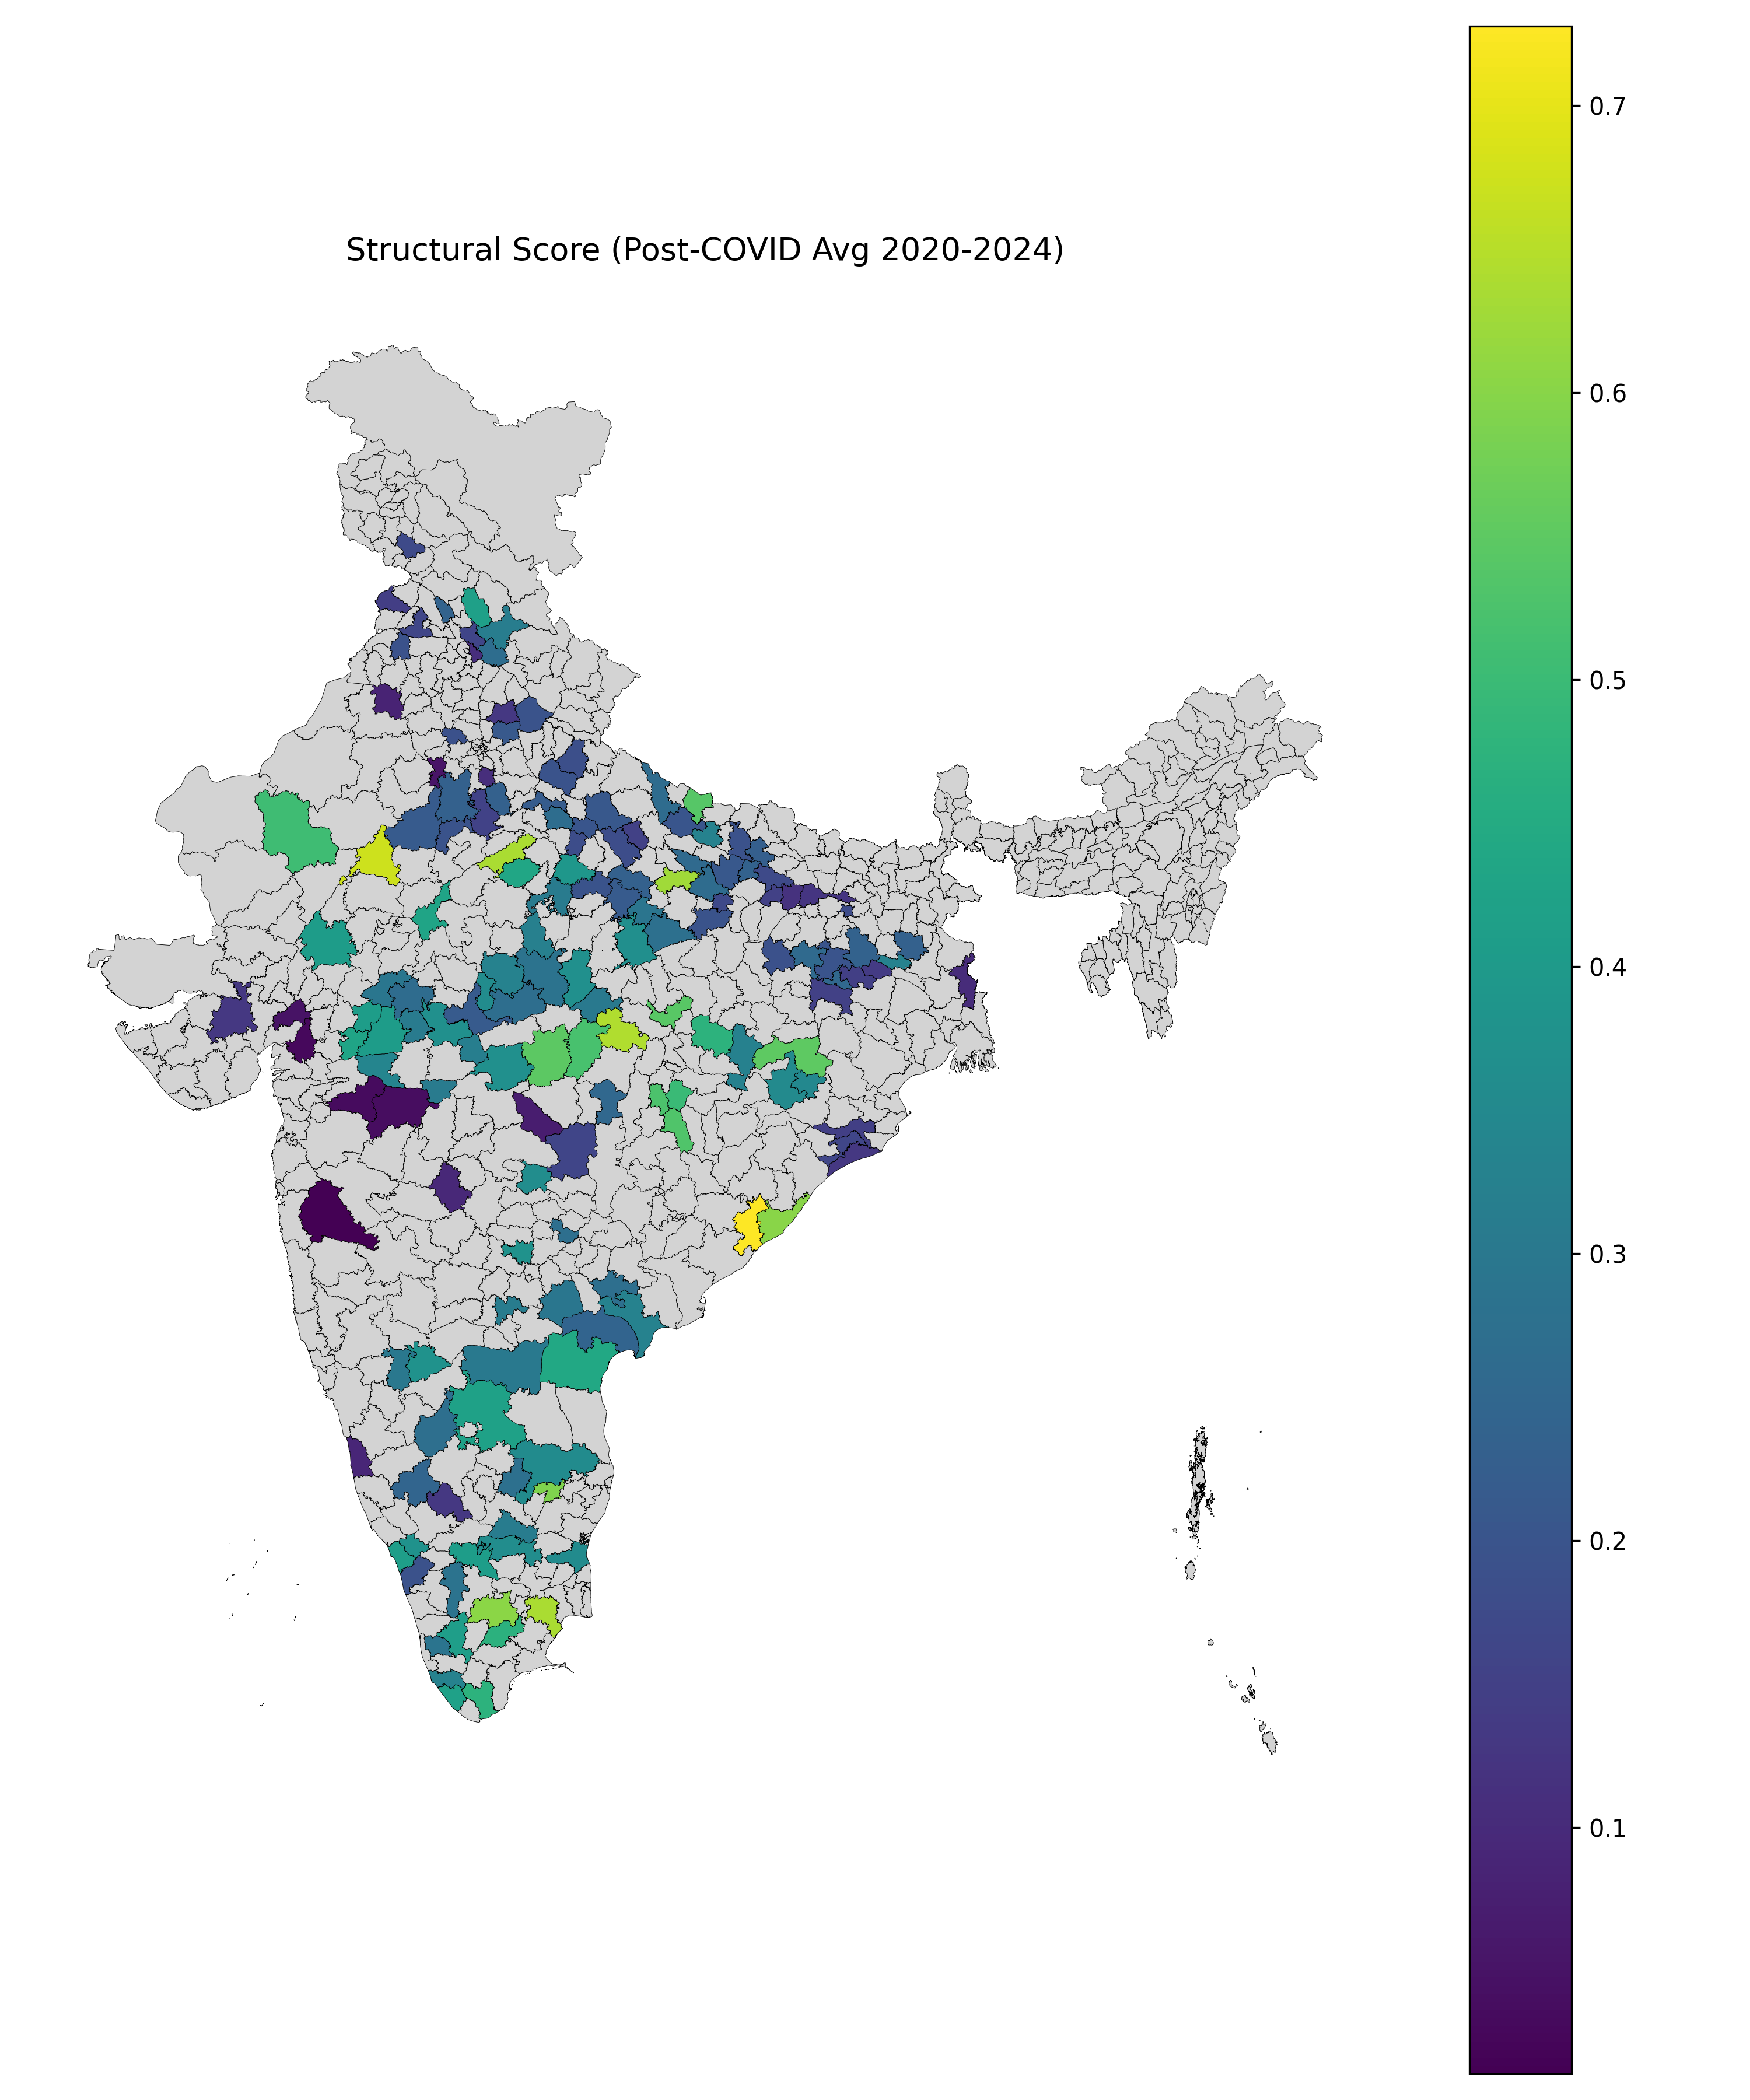
\includegraphics[width=0.85\textwidth]{figures/india_structural_map.png}
\caption{Structural persistence scores across districts.}
\end{figure}

These maps provide additional spatial detail and highlight the variation in program performance across different dimensions.


\section{Robustness Checks and Diagnostics}

To ensure the reliability of the results, several diagnostic checks are performed.

\subsection{Correlation Across Pillars}

The correlation matrix shows that the pillars are not perfectly correlated, indicating that each dimension captures distinct aspects of program performance.

\subsection{Variance of Pillars}

All constructed pillars exhibit sufficient variation across districts and time, ensuring that the composite index is not driven by a single dimension.

\subsection{Alternative Specifications}

The results remain broadly consistent under alternative specifications, including:

\begin{itemize}
\item Different normalization methods
\item Exclusion of extreme observations
\item Separate estimation for pre- and post-COVID periods
\end{itemize}

These checks suggest that the main findings are robust to reasonable changes in model specification.


\section{Variable Definitions}

This section provides a summary of key variables used in the analysis.

\begin{table}[H]
\centering
\setlength{\tabcolsep}{10pt}
\renewcommand{\arraystretch}{1.25}
\begin{tabularx}{\textwidth}{>{\raggedright\arraybackslash\bfseries}p{0.30\textwidth} >{\raggedright\arraybackslash}X}
\toprule
\rowcolor{black!8}
\textbf{Variable} & \textbf{Description} \\
\midrule
MGNREGA & Program intensity (employment or expenditure proxy) \\
Income & District-level aggregated income \\
Consumption & District-level consumption expenditure \\
Yield & Agricultural productivity (output per unit area) \\
Rainfall & Annual rainfall (mm) \\
Shock & Deviation from average rainfall \\
Distribution & Participation of marginalized groups (SC/ST, women) \\
Distortion & Ratio of income effect to productivity effect \\
Structural & Lagged impact of MGNREGA on income \\
Composite Index & Average of normalized pillar scores \\
\bottomrule
\end{tabularx}
\caption{Definition of key variables}
\end{table}

This table provides a concise reference for the variables used throughout the paper.



\newpage

\section{References}

% At the end of document (replace manual bibliography)
\bibliographystyle{apalike}
\bibliography{references}

\end{document}
